\documentclass[twoside]{book}

% Packages required by doxygen
\usepackage{fixltx2e}
\usepackage{calc}
\usepackage{doxygen}
\usepackage[export]{adjustbox} % also loads graphicx
\usepackage{graphicx}
\usepackage[utf8]{inputenc}
\usepackage{makeidx}
\usepackage{multicol}
\usepackage{multirow}
\PassOptionsToPackage{warn}{textcomp}
\usepackage{textcomp}
\usepackage[nointegrals]{wasysym}
\usepackage[table]{xcolor}

% NLS support packages
\usepackage[brazil]{babel}
% Font selection
\usepackage[T1]{fontenc}
\usepackage[scaled=.90]{helvet}
\usepackage{courier}
\usepackage{amssymb}
\usepackage{sectsty}
\renewcommand{\familydefault}{\sfdefault}
\allsectionsfont{%
  \fontseries{bc}\selectfont%
  \color{darkgray}%
}
\renewcommand{\DoxyLabelFont}{%
  \fontseries{bc}\selectfont%
  \color{darkgray}%
}
\newcommand{\+}{\discretionary{\mbox{\scriptsize$\hookleftarrow$}}{}{}}

% Page & text layout
\usepackage{geometry}
\geometry{%
  a4paper,%
  top=2.5cm,%
  bottom=2.5cm,%
  left=2.5cm,%
  right=2.5cm%
}
\tolerance=750
\hfuzz=15pt
\hbadness=750
\setlength{\emergencystretch}{15pt}
\setlength{\parindent}{0cm}
\setlength{\parskip}{3ex plus 2ex minus 2ex}
\makeatletter
\renewcommand{\paragraph}{%
  \@startsection{paragraph}{4}{0ex}{-1.0ex}{1.0ex}{%
    \normalfont\normalsize\bfseries\SS@parafont%
  }%
}
\renewcommand{\subparagraph}{%
  \@startsection{subparagraph}{5}{0ex}{-1.0ex}{1.0ex}{%
    \normalfont\normalsize\bfseries\SS@subparafont%
  }%
}
\makeatother

% Headers & footers
\usepackage{fancyhdr}
\pagestyle{fancyplain}
\fancyhead[LE]{\fancyplain{}{\bfseries\thepage}}
\fancyhead[CE]{\fancyplain{}{}}
\fancyhead[RE]{\fancyplain{}{\bfseries\leftmark}}
\fancyhead[LO]{\fancyplain{}{\bfseries\rightmark}}
\fancyhead[CO]{\fancyplain{}{}}
\fancyhead[RO]{\fancyplain{}{\bfseries\thepage}}
\fancyfoot[LE]{\fancyplain{}{}}
\fancyfoot[CE]{\fancyplain{}{}}
\fancyfoot[RE]{\fancyplain{}{\bfseries\scriptsize Gerado por Doxygen }}
\fancyfoot[LO]{\fancyplain{}{\bfseries\scriptsize Gerado por Doxygen }}
\fancyfoot[CO]{\fancyplain{}{}}
\fancyfoot[RO]{\fancyplain{}{}}
\renewcommand{\footrulewidth}{0.4pt}
\renewcommand{\chaptermark}[1]{%
  \markboth{#1}{}%
}
\renewcommand{\sectionmark}[1]{%
  \markright{\thesection\ #1}%
}

% Indices & bibliography
\usepackage{natbib}
\usepackage[titles]{tocloft}
\setcounter{tocdepth}{3}
\setcounter{secnumdepth}{5}
\makeindex

% Hyperlinks (required, but should be loaded last)
\usepackage{ifpdf}
\ifpdf
  \usepackage[pdftex,pagebackref=true]{hyperref}
\else
  \usepackage[ps2pdf,pagebackref=true]{hyperref}
\fi
\hypersetup{%
  colorlinks=true,%
  linkcolor=blue,%
  citecolor=blue,%
  unicode%
}

% Custom commands
\newcommand{\clearemptydoublepage}{%
  \newpage{\pagestyle{empty}\cleardoublepage}%
}

\usepackage{caption}
\captionsetup{labelsep=space,justification=centering,font={bf},singlelinecheck=off,skip=4pt,position=top}

%===== C O N T E N T S =====

\begin{document}

% Titlepage & ToC
\hypersetup{pageanchor=false,
             bookmarksnumbered=true,
             pdfencoding=unicode
            }
\pagenumbering{alph}
\begin{titlepage}
\vspace*{7cm}
\begin{center}%
{\Large U\+DP Tic-\/\+Tac-\/\+Toe }\\
\vspace*{1cm}
{\large Gerado por Doxygen 1.8.13}\\
\end{center}
\end{titlepage}
\clearemptydoublepage
\pagenumbering{roman}
\tableofcontents
\clearemptydoublepage
\pagenumbering{arabic}
\hypersetup{pageanchor=true}

%--- Begin generated contents ---
\chapter{Índice das Estruturas de Dados}
\section{Estruturas de Dados}
Aqui estão as estruturas de dados, uniões e suas respectivas descrições\+:\begin{DoxyCompactList}
\item\contentsline{section}{\hyperlink{structgame}{game} }{\pageref{structgame}}{}
\item\contentsline{section}{\hyperlink{structmessagem}{messagem} }{\pageref{structmessagem}}{}
\item\contentsline{section}{\hyperlink{structplayer}{player} }{\pageref{structplayer}}{}
\item\contentsline{section}{\hyperlink{structreceived__message}{received\+\_\+message} }{\pageref{structreceived__message}}{}
\end{DoxyCompactList}

\chapter{Índice dos Arquivos}
\section{Lista de Arquivos}
Esta é a lista de todos os arquivos documentados e suas respectivas descrições\+:\begin{DoxyCompactList}
\item\contentsline{section}{client/include/\hyperlink{board_8h}{board.\+h} \\*Arquivo contendo as estruturas e cabeçalhos de funções do tabuleiro }{\pageref{board_8h}}{}
\item\contentsline{section}{client/include/\hyperlink{client_8h}{client.\+h} \\*Arquivo contendo as estruturas e cabeçalhos de funções do cliente }{\pageref{client_8h}}{}
\item\contentsline{section}{client/include/\hyperlink{game_8h}{game.\+h} \\*Arquivo contendo as estruturas e cabeçalhos de funções do jogo }{\pageref{game_8h}}{}
\item\contentsline{section}{client/include/\hyperlink{menu_8h}{menu.\+h} \\*Arquivo contendo as estruturas e cabeçalhos de funções do menu }{\pageref{menu_8h}}{}
\item\contentsline{section}{client/include/\hyperlink{player_8h}{player.\+h} \\*Arquivo contendo cabeçalhos de funções que implementam as funções do player }{\pageref{player_8h}}{}
\item\contentsline{section}{server/include/\hyperlink{client__thread_8h}{client\+\_\+thread.\+h} \\*Arquivo contendo cabeçalhos de funções que implementam as interações do servidor com os clientes conectados }{\pageref{client__thread_8h}}{}
\item\contentsline{section}{server/include/\hyperlink{server_8h}{server.\+h} \\*Arquivo contendo as estruturas e cabeçalhos de funções do servidor }{\pageref{server_8h}}{}
\item\contentsline{section}{server/src/\hyperlink{client__thread_8c}{client\+\_\+thread.\+c} \\*Implementação das funções de conexão via thread dedicada }{\pageref{client__thread_8c}}{}
\item\contentsline{section}{server/src/\hyperlink{server_8c}{server.\+c} \\*Implementação das funções do servidor }{\pageref{server_8c}}{}
\end{DoxyCompactList}

\chapter{Estruturas}
\hypertarget{structgame}{}\section{Referência da Estrutura game}
\label{structgame}\index{game@{game}}


Diagrama de colaboração para game\+:
\nopagebreak
\begin{figure}[H]
\begin{center}
\leavevmode
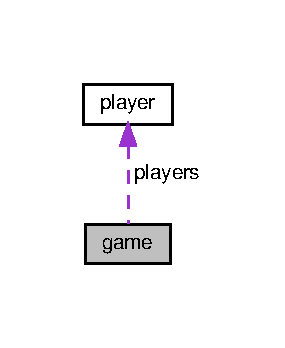
\includegraphics[width=137pt]{structgame__coll__graph}
\end{center}
\end{figure}
\subsection*{Campos de Dados}
\begin{DoxyCompactItemize}
\item 
\hyperlink{server_8h_a9c8780378078e51e7c9041cbac392db9}{Player} \hyperlink{structgame_a61d36a149f0d4d23b4ec8bff3a256d9f}{players} \mbox{[}2\mbox{]}
\item 
unsigned short \hyperlink{structgame_a92e543c2bad8ce842e762eb639b7ae66}{number\+\_\+of\+\_\+players}
\item 
int \hyperlink{structgame_aa1fa2aa40af4537744fa6b0a0ae4227c}{first\+\_\+player}
\end{DoxyCompactItemize}


\subsection{Campos}
\mbox{\Hypertarget{structgame_aa1fa2aa40af4537744fa6b0a0ae4227c}\label{structgame_aa1fa2aa40af4537744fa6b0a0ae4227c}} 
\index{game@{game}!first\+\_\+player@{first\+\_\+player}}
\index{first\+\_\+player@{first\+\_\+player}!game@{game}}
\subsubsection{\texorpdfstring{first\+\_\+player}{first\_player}}
{\footnotesize\ttfamily int game\+::first\+\_\+player}

Armazena o id do jogador que começará/começou jogando essa partida. \mbox{\Hypertarget{structgame_a92e543c2bad8ce842e762eb639b7ae66}\label{structgame_a92e543c2bad8ce842e762eb639b7ae66}} 
\index{game@{game}!number\+\_\+of\+\_\+players@{number\+\_\+of\+\_\+players}}
\index{number\+\_\+of\+\_\+players@{number\+\_\+of\+\_\+players}!game@{game}}
\subsubsection{\texorpdfstring{number\+\_\+of\+\_\+players}{number\_of\_players}}
{\footnotesize\ttfamily unsigned short game\+::number\+\_\+of\+\_\+players}

Armazena o número de jogadores conectados a essa partida. \mbox{\Hypertarget{structgame_a61d36a149f0d4d23b4ec8bff3a256d9f}\label{structgame_a61d36a149f0d4d23b4ec8bff3a256d9f}} 
\index{game@{game}!players@{players}}
\index{players@{players}!game@{game}}
\subsubsection{\texorpdfstring{players}{players}}
{\footnotesize\ttfamily \hyperlink{server_8h_a9c8780378078e51e7c9041cbac392db9}{Player} game\+::players\mbox{[}2\mbox{]}}

Array contendo os jogadores atualmente nessa partida. 

A documentação para esta estrutura foi gerada a partir do seguinte arquivo\+:\begin{DoxyCompactItemize}
\item 
server/include/\hyperlink{server_8h}{server.\+h}\end{DoxyCompactItemize}

\hypertarget{structmessagem}{}\section{Referência da Estrutura messagem}
\label{structmessagem}\index{messagem@{messagem}}
\subsection*{Campos de Dados}
\begin{DoxyCompactItemize}
\item 
char \hyperlink{structmessagem_a23e2fc404fdd389c4ff6da925ab4ae21}{data} \mbox{[}T\+A\+M\+\_\+\+M\+SG\mbox{]}
\item 
struct sockaddr\+\_\+in \hyperlink{structmessagem_af4f1e53a419d163b87b5c4d510fb5a0f}{client\+\_\+addr}
\end{DoxyCompactItemize}


\subsection{Campos}
\mbox{\Hypertarget{structmessagem_af4f1e53a419d163b87b5c4d510fb5a0f}\label{structmessagem_af4f1e53a419d163b87b5c4d510fb5a0f}} 
\index{messagem@{messagem}!client\+\_\+addr@{client\+\_\+addr}}
\index{client\+\_\+addr@{client\+\_\+addr}!messagem@{messagem}}
\subsubsection{\texorpdfstring{client\+\_\+addr}{client\_addr}}
{\footnotesize\ttfamily struct sockaddr\+\_\+in messagem\+::client\+\_\+addr}

Endereço do remetente da mensagem \mbox{\Hypertarget{structmessagem_a23e2fc404fdd389c4ff6da925ab4ae21}\label{structmessagem_a23e2fc404fdd389c4ff6da925ab4ae21}} 
\index{messagem@{messagem}!data@{data}}
\index{data@{data}!messagem@{messagem}}
\subsubsection{\texorpdfstring{data}{data}}
{\footnotesize\ttfamily char messagem\+::data\mbox{[}T\+A\+M\+\_\+\+M\+SG\mbox{]}}

Conteúdo da mensagem recebida. 

A documentação para esta estrutura foi gerada a partir do seguinte arquivo\+:\begin{DoxyCompactItemize}
\item 
client/include/\hyperlink{client_8h}{client.\+h}\end{DoxyCompactItemize}

\hypertarget{structplayer}{}\section{Referência da Estrutura player}
\label{structplayer}\index{player@{player}}
\subsection*{Campos de Dados}
\begin{DoxyCompactItemize}
\item 
unsigned short \hyperlink{structplayer_a0e6fb0e744015cdf9f4dd12164a1dbaa}{id}
\item 
char \hyperlink{structplayer_a6db5a6f2e823dfebcbc3548bfb4bda99}{name} \mbox{[}64\mbox{]}
\item 
\hyperlink{server_8h_a2645d40a71683d956e55bcf7a6823530}{Sockaddr} \hyperlink{structplayer_a7b6c5d24a563be91d800cd5ed7d639e1}{addr}
\end{DoxyCompactItemize}


\subsection{Campos}
\mbox{\Hypertarget{structplayer_a7b6c5d24a563be91d800cd5ed7d639e1}\label{structplayer_a7b6c5d24a563be91d800cd5ed7d639e1}} 
\index{player@{player}!addr@{addr}}
\index{addr@{addr}!player@{player}}
\subsubsection{\texorpdfstring{addr}{addr}}
{\footnotesize\ttfamily \hyperlink{server_8h_a2645d40a71683d956e55bcf7a6823530}{Sockaddr} player\+::addr}

Endereço remoto do jogador. \mbox{\Hypertarget{structplayer_a0e6fb0e744015cdf9f4dd12164a1dbaa}\label{structplayer_a0e6fb0e744015cdf9f4dd12164a1dbaa}} 
\index{player@{player}!id@{id}}
\index{id@{id}!player@{player}}
\subsubsection{\texorpdfstring{id}{id}}
{\footnotesize\ttfamily unsigned short player\+::id}

id do jogador dentro de uma partida, podendo ser 1 ou 0. \mbox{\Hypertarget{structplayer_a6db5a6f2e823dfebcbc3548bfb4bda99}\label{structplayer_a6db5a6f2e823dfebcbc3548bfb4bda99}} 
\index{player@{player}!name@{name}}
\index{name@{name}!player@{player}}
\subsubsection{\texorpdfstring{name}{name}}
{\footnotesize\ttfamily char player\+::name\mbox{[}64\mbox{]}}

Nome do jogador. 

A documentação para esta estrutura foi gerada a partir do seguinte arquivo\+:\begin{DoxyCompactItemize}
\item 
server/include/\hyperlink{server_8h}{server.\+h}\end{DoxyCompactItemize}

\hypertarget{structreceived__message}{}\section{Referência da Estrutura received\+\_\+message}
\label{structreceived__message}\index{received\+\_\+message@{received\+\_\+message}}
\subsection*{Campos de Dados}
\begin{DoxyCompactItemize}
\item 
char \hyperlink{structreceived__message_ada9c34d3c26df419fa3dd0ac2c20e860}{data} \mbox{[}T\+A\+M\+\_\+\+M\+SG\mbox{]}
\item 
\hyperlink{server_8h_a2645d40a71683d956e55bcf7a6823530}{Sockaddr} \hyperlink{structreceived__message_ad56a4c16bef95bef52ac591efe2582ec}{client\+\_\+addr}
\end{DoxyCompactItemize}


\subsection{Campos}
\mbox{\Hypertarget{structreceived__message_ad56a4c16bef95bef52ac591efe2582ec}\label{structreceived__message_ad56a4c16bef95bef52ac591efe2582ec}} 
\index{received\+\_\+message@{received\+\_\+message}!client\+\_\+addr@{client\+\_\+addr}}
\index{client\+\_\+addr@{client\+\_\+addr}!received\+\_\+message@{received\+\_\+message}}
\subsubsection{\texorpdfstring{client\+\_\+addr}{client\_addr}}
{\footnotesize\ttfamily \hyperlink{server_8h_a2645d40a71683d956e55bcf7a6823530}{Sockaddr} received\+\_\+message\+::client\+\_\+addr}

Endereço do remetente da mensagem \mbox{\Hypertarget{structreceived__message_ada9c34d3c26df419fa3dd0ac2c20e860}\label{structreceived__message_ada9c34d3c26df419fa3dd0ac2c20e860}} 
\index{received\+\_\+message@{received\+\_\+message}!data@{data}}
\index{data@{data}!received\+\_\+message@{received\+\_\+message}}
\subsubsection{\texorpdfstring{data}{data}}
{\footnotesize\ttfamily char received\+\_\+message\+::data\mbox{[}T\+A\+M\+\_\+\+M\+SG\mbox{]}}

Conteúdo da mensagem recebida. 

A documentação para esta estrutura foi gerada a partir do seguinte arquivo\+:\begin{DoxyCompactItemize}
\item 
server/include/\hyperlink{server_8h}{server.\+h}\end{DoxyCompactItemize}

\chapter{Arquivos}
\hypertarget{board_8h}{}\section{Referência do Arquivo client/include/board.h}
\label{board_8h}\index{client/include/board.\+h@{client/include/board.\+h}}


Arquivo contendo as estruturas e cabeçalhos de funções do tabuleiro.  


{\ttfamily \#include $<$stdio.\+h$>$}\newline
{\ttfamily \#include $<$stdlib.\+h$>$}\newline
Gráfico de dependência de inclusões para board.\+h\+:
\nopagebreak
\begin{figure}[H]
\begin{center}
\leavevmode
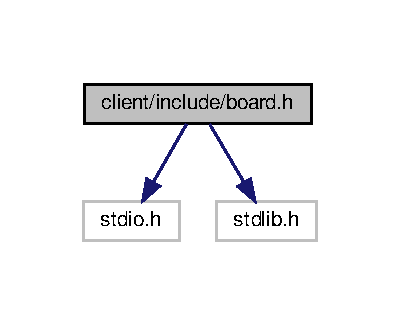
\includegraphics[width=192pt]{board_8h__incl}
\end{center}
\end{figure}
Este grafo mostra quais arquivos estão direta ou indiretamente relacionados com este arquivo\+:
\nopagebreak
\begin{figure}[H]
\begin{center}
\leavevmode
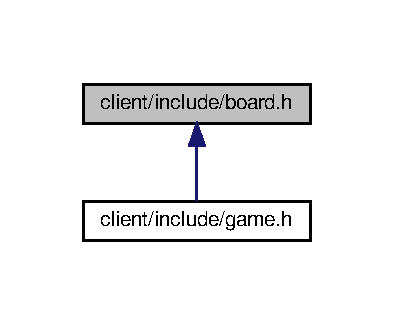
\includegraphics[width=189pt]{board_8h__dep__incl}
\end{center}
\end{figure}
\subsection*{Funções}
\begin{DoxyCompactItemize}
\item 
void \hyperlink{board_8h_a59e294ac28318369e0f8c7e50c6ae488}{Draw\+Board} (char game\+Board\mbox{[}9\mbox{]})
\begin{DoxyCompactList}\small\item\em Constroi o tabuleiro do jogo. \end{DoxyCompactList}\item 
void \hyperlink{board_8h_abb7dab68efbd40aaffe686a1b65eb6ce}{Draw\+Board\+With\+Names} (char game\+Board\mbox{[}9\mbox{]}, char $\ast$player1\+Name, char $\ast$player2\+Name, char $\ast$player\+Character)
\begin{DoxyCompactList}\small\item\em Constroi o tabuleiro do jogo. \end{DoxyCompactList}\item 
int \hyperlink{board_8h_a8faf24edc7214b49027b34cdae00293d}{Check\+Player\+Win} (char game\+Board\mbox{[}9\mbox{]})
\begin{DoxyCompactList}\small\item\em Constroi o tabuleiro do jogo. \end{DoxyCompactList}\item 
int \hyperlink{board_8h_a04497f61d533bce8e10181d659317f65}{check\+Valid\+Play} (char $\ast$game\+Board, int position)
\begin{DoxyCompactList}\small\item\em Verifica a jogada. \end{DoxyCompactList}\item 
void \hyperlink{board_8h_abc40cd622f423abf44084c8f8595f57f}{clear\+\_\+screen} (void)
\begin{DoxyCompactList}\small\item\em Limpa a tela. \end{DoxyCompactList}\end{DoxyCompactItemize}


\subsection{Descrição Detalhada}
Arquivo contendo as estruturas e cabeçalhos de funções do tabuleiro. 

\begin{DoxyAuthor}{Autor}
Vitor Correa da Silva 
\end{DoxyAuthor}
\begin{DoxyDate}{Data}
29 May 2020
\end{DoxyDate}
Esse arquivo contém as definições das funções que são implementadas em board.\+c. Essas funções tem como objetivo implementar o tabuleiro do jogo e suas especificações. 

\subsection{Funções}
\mbox{\Hypertarget{board_8h_a8faf24edc7214b49027b34cdae00293d}\label{board_8h_a8faf24edc7214b49027b34cdae00293d}} 
\index{board.\+h@{board.\+h}!Check\+Player\+Win@{Check\+Player\+Win}}
\index{Check\+Player\+Win@{Check\+Player\+Win}!board.\+h@{board.\+h}}
\subsubsection{\texorpdfstring{Check\+Player\+Win()}{CheckPlayerWin()}}
{\footnotesize\ttfamily int Check\+Player\+Win (\begin{DoxyParamCaption}\item[{char}]{game\+Board\mbox{[}9\mbox{]} }\end{DoxyParamCaption})}



Constroi o tabuleiro do jogo. 

Verifica se houve uma vitoria (1), empate (2) ou se o jogo continua (0)


\begin{DoxyParams}{Parâmetros}
{\em game\+Board} & Array de 9 posições que guarda as informações do tabuleiro \\
\hline
\end{DoxyParams}
\begin{DoxyReturn}{Retorna}
{\ttfamily int} Verifica se a jogada foi a vencedora 
\end{DoxyReturn}
\mbox{\Hypertarget{board_8h_a04497f61d533bce8e10181d659317f65}\label{board_8h_a04497f61d533bce8e10181d659317f65}} 
\index{board.\+h@{board.\+h}!check\+Valid\+Play@{check\+Valid\+Play}}
\index{check\+Valid\+Play@{check\+Valid\+Play}!board.\+h@{board.\+h}}
\subsubsection{\texorpdfstring{check\+Valid\+Play()}{checkValidPlay()}}
{\footnotesize\ttfamily int check\+Valid\+Play (\begin{DoxyParamCaption}\item[{char $\ast$}]{game\+Board,  }\item[{int}]{position }\end{DoxyParamCaption})}



Verifica a jogada. 

Verifica se a jogada feita é valida.


\begin{DoxyParams}{Parâmetros}
{\em game\+Board} & Array de 9 posições que guarda as informações do tabuleiro \\
\hline
{\em position} & Valor da possivel jogada \\
\hline
\end{DoxyParams}
\begin{DoxyReturn}{Retorna}
{\ttfamily int} retorna a jogada feita se for valida 
\end{DoxyReturn}
\mbox{\Hypertarget{board_8h_abc40cd622f423abf44084c8f8595f57f}\label{board_8h_abc40cd622f423abf44084c8f8595f57f}} 
\index{board.\+h@{board.\+h}!clear\+\_\+screen@{clear\+\_\+screen}}
\index{clear\+\_\+screen@{clear\+\_\+screen}!board.\+h@{board.\+h}}
\subsubsection{\texorpdfstring{clear\+\_\+screen()}{clear\_screen()}}
{\footnotesize\ttfamily void clear\+\_\+screen (\begin{DoxyParamCaption}\item[{void}]{ }\end{DoxyParamCaption})}



Limpa a tela. 

Implementa função para lipar a tela. \mbox{\Hypertarget{board_8h_a59e294ac28318369e0f8c7e50c6ae488}\label{board_8h_a59e294ac28318369e0f8c7e50c6ae488}} 
\index{board.\+h@{board.\+h}!Draw\+Board@{Draw\+Board}}
\index{Draw\+Board@{Draw\+Board}!board.\+h@{board.\+h}}
\subsubsection{\texorpdfstring{Draw\+Board()}{DrawBoard()}}
{\footnotesize\ttfamily void Draw\+Board (\begin{DoxyParamCaption}\item[{char}]{game\+Board\mbox{[}9\mbox{]} }\end{DoxyParamCaption})}



Constroi o tabuleiro do jogo. 

Limpa a tela e desenha o tabuleiro de jogo.


\begin{DoxyParams}{Parâmetros}
{\em game\+Board} & Array de 9 posições que guarda as informações do tabuleiro \\
\hline
\end{DoxyParams}
\mbox{\Hypertarget{board_8h_abb7dab68efbd40aaffe686a1b65eb6ce}\label{board_8h_abb7dab68efbd40aaffe686a1b65eb6ce}} 
\index{board.\+h@{board.\+h}!Draw\+Board\+With\+Names@{Draw\+Board\+With\+Names}}
\index{Draw\+Board\+With\+Names@{Draw\+Board\+With\+Names}!board.\+h@{board.\+h}}
\subsubsection{\texorpdfstring{Draw\+Board\+With\+Names()}{DrawBoardWithNames()}}
{\footnotesize\ttfamily void Draw\+Board\+With\+Names (\begin{DoxyParamCaption}\item[{char}]{game\+Board\mbox{[}9\mbox{]},  }\item[{char $\ast$}]{player1\+Name,  }\item[{char $\ast$}]{player2\+Name,  }\item[{char $\ast$}]{player\+Character }\end{DoxyParamCaption})}



Constroi o tabuleiro do jogo. 

Limpa a tela, desenha o tabuleiro e informa de qual jogador é a vez.


\begin{DoxyParams}{Parâmetros}
{\em game\+Board} & Array de 9 posições que guarda as informações do tabuleiro \\
\hline
{\em player1\+Name} & Nome do jogador numero 1 \\
\hline
{\em player2\+Name} & Nome do jogador numero 2 \\
\hline
{\em player\+Character} & Caractere do jogador atual \\
\hline
\end{DoxyParams}

\hypertarget{client_8h}{}\section{Referência do Arquivo client/include/client.h}
\label{client_8h}\index{client/include/client.\+h@{client/include/client.\+h}}


Arquivo contendo as estruturas e cabeçalhos de funções do cliente.  


{\ttfamily \#include $<$sys/types.\+h$>$}\newline
{\ttfamily \#include $<$sys/socket.\+h$>$}\newline
{\ttfamily \#include $<$netinet/in.\+h$>$}\newline
{\ttfamily \#include $<$unistd.\+h$>$}\newline
{\ttfamily \#include $<$arpa/inet.\+h$>$}\newline
{\ttfamily \#include $<$netdb.\+h$>$}\newline
{\ttfamily \#include $<$signal.\+h$>$}\newline
{\ttfamily \#include $<$stdio.\+h$>$}\newline
{\ttfamily \#include $<$string.\+h$>$}\newline
{\ttfamily \#include $<$fcntl.\+h$>$}\newline
{\ttfamily \#include $<$errno.\+h$>$}\newline
{\ttfamily \#include $<$sys/time.\+h$>$}\newline
{\ttfamily \#include $<$stdlib.\+h$>$}\newline
{\ttfamily \#include $<$memory.\+h$>$}\newline
{\ttfamily \#include $<$ifaddrs.\+h$>$}\newline
{\ttfamily \#include $<$net/if.\+h$>$}\newline
{\ttfamily \#include $<$stdarg.\+h$>$}\newline
{\ttfamily \#include $<$time.\+h$>$}\newline
{\ttfamily \#include $<$math.\+h$>$}\newline
{\ttfamily \#include $<$sys/termios.\+h$>$}\newline
{\ttfamily \#include $<$menu.\+h$>$}\newline
Gráfico de dependência de inclusões para client.\+h\+:
\nopagebreak
\begin{figure}[H]
\begin{center}
\leavevmode
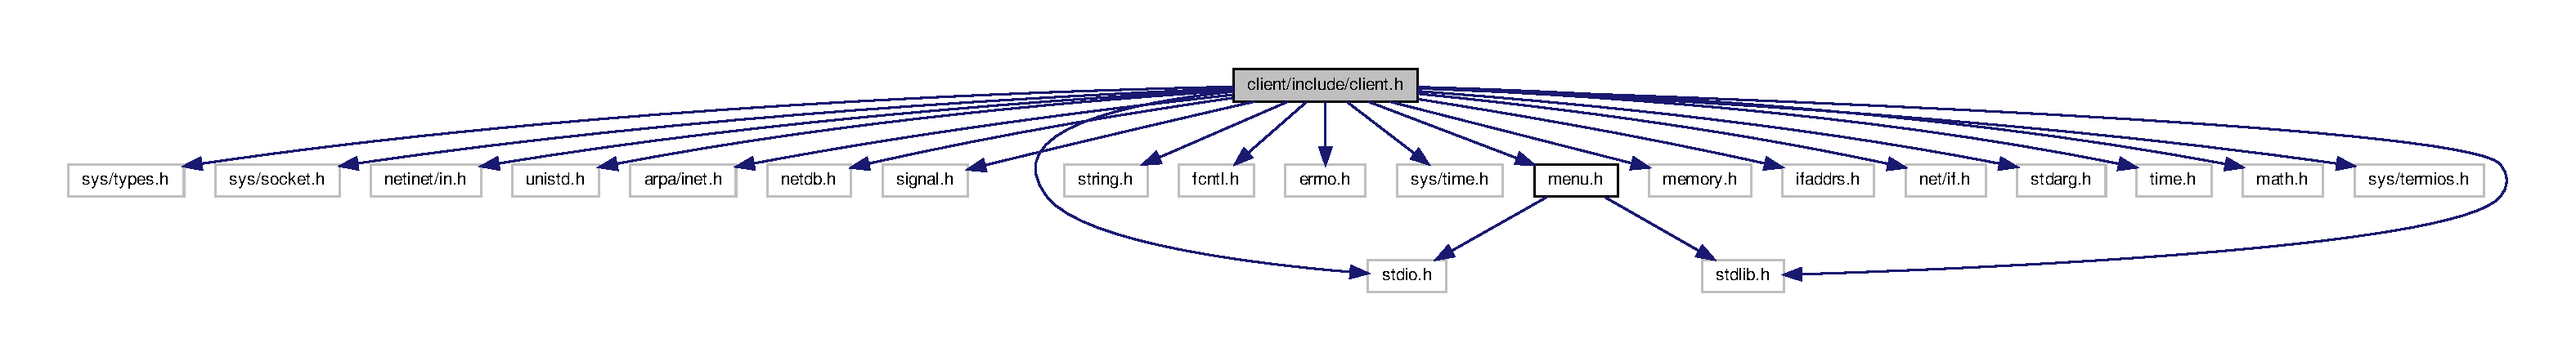
\includegraphics[width=350pt]{client_8h__incl}
\end{center}
\end{figure}
\subsection*{Estruturas de Dados}
\begin{DoxyCompactItemize}
\item 
struct \hyperlink{structmessagem}{messagem}
\end{DoxyCompactItemize}
\subsection*{Definições e Macros}
\begin{DoxyCompactItemize}
\item 
\mbox{\Hypertarget{client_8h_a4af527b772cacbae6d6a0e48c3dcf53f}\label{client_8h_a4af527b772cacbae6d6a0e48c3dcf53f}} 
\#define {\bfseries T\+A\+M\+\_\+\+M\+SG}~1024
\end{DoxyCompactItemize}
\subsection*{Definições de Tipos}
\begin{DoxyCompactItemize}
\item 
typedef struct \hyperlink{structmessagem}{messagem} \hyperlink{client_8h_a13d6eab42ea1147a3b4b74bbec7a336b}{Mensagem}
\begin{DoxyCompactList}\small\item\em Mensagem recebida. \end{DoxyCompactList}\end{DoxyCompactItemize}
\subsection*{Funções}
\begin{DoxyCompactItemize}
\item 
int \hyperlink{client_8h_ad38905c5727913b84d4ba2c3982c03dc}{create\+\_\+client\+\_\+socket} (void)
\begin{DoxyCompactList}\small\item\em Cria um socket udp. \end{DoxyCompactList}\item 
int \hyperlink{client_8h_a1ab0d52a5f583e6f915a9dba47c951dd}{rand\+\_\+range} (int min, int max)
\begin{DoxyCompactList}\small\item\em Gerador de número aleatório dentro de um intervalo. \end{DoxyCompactList}\item 
\hyperlink{client_8h_a13d6eab42ea1147a3b4b74bbec7a336b}{Mensagem} \hyperlink{client_8h_adef25c5e886373a98ba508568deb2d8a}{receive\+\_\+message} (int sockfd)
\begin{DoxyCompactList}\small\item\em Espera pela chegada de uma mensagem em um socket. \end{DoxyCompactList}\item 
int \hyperlink{client_8h_a7f26bc4fe6b5efd6b64e1edc39b7465c}{envia\+\_\+mensagem} (int socketfd, char $\ast$msg, char $\ast$host, int port)
\begin{DoxyCompactList}\small\item\em Envia uma mensagem para um endereço via socket udp. \end{DoxyCompactList}\item 
int \hyperlink{client_8h_a183fbb1ab8be41f5bf8011b67bca7c20}{login} (int socket, char $\ast$host, int port)
\begin{DoxyCompactList}\small\item\em Realiza o login no servidor. \end{DoxyCompactList}\item 
\mbox{\Hypertarget{client_8h_afb06e752d0facf30119fa60471bce565}\label{client_8h_afb06e752d0facf30119fa60471bce565}} 
int \hyperlink{client_8h_afb06e752d0facf30119fa60471bce565}{play\+\_\+tictactoe} (int socket, char $\ast$host, int port)
\begin{DoxyCompactList}\small\item\em Implementa com o uso das outras funções o jogo. \end{DoxyCompactList}\item 
void \hyperlink{client_8h_af5fb66f96b329174a0e8887f9209da5b}{clear\+\_\+stdin} (void)
\begin{DoxyCompactList}\small\item\em Limpa caracteres. \end{DoxyCompactList}\item 
void \hyperlink{client_8h_aebd00ba894071e030e959c4b18353634}{disconnect} (int socket, char $\ast$host, int port)
\begin{DoxyCompactList}\small\item\em Desconecta do socket. \end{DoxyCompactList}\end{DoxyCompactItemize}


\subsection{Descrição Detalhada}
Arquivo contendo as estruturas e cabeçalhos de funções do cliente. 

\begin{DoxyAuthor}{Autor}
Vitor Correa da Silva 
\end{DoxyAuthor}
\begin{DoxyDate}{Data}
29 May 2020
\end{DoxyDate}
Esse arquivo contém as definições das funções que são implementadas em client.\+c. Essas funções tem como objetivo implementar um client udp que faz login no servidor, envia e recebe mensagens. 

\subsection{Definições dos tipos}
\mbox{\Hypertarget{client_8h_a13d6eab42ea1147a3b4b74bbec7a336b}\label{client_8h_a13d6eab42ea1147a3b4b74bbec7a336b}} 
\index{client.\+h@{client.\+h}!Mensagem@{Mensagem}}
\index{Mensagem@{Mensagem}!client.\+h@{client.\+h}}
\subsubsection{\texorpdfstring{Mensagem}{Mensagem}}
{\footnotesize\ttfamily \hyperlink{client_8h_a13d6eab42ea1147a3b4b74bbec7a336b}{Mensagem}}



Mensagem recebida. 

Mensagem guarda o conteúdo e informações referentes a uma mensagem recebida via socket U\+DP. 

\subsection{Funções}
\mbox{\Hypertarget{client_8h_af5fb66f96b329174a0e8887f9209da5b}\label{client_8h_af5fb66f96b329174a0e8887f9209da5b}} 
\index{client.\+h@{client.\+h}!clear\+\_\+stdin@{clear\+\_\+stdin}}
\index{clear\+\_\+stdin@{clear\+\_\+stdin}!client.\+h@{client.\+h}}
\subsubsection{\texorpdfstring{clear\+\_\+stdin()}{clear\_stdin()}}
{\footnotesize\ttfamily void clear\+\_\+stdin (\begin{DoxyParamCaption}\item[{void}]{ }\end{DoxyParamCaption})}



Limpa caracteres. 

Limpa as entradas de teclado desnecessarias que ficam salvas depois que é realizado o scanf


\begin{DoxyParams}{Parâmetros}
{\em void} & Não há parametros \\
\hline
\end{DoxyParams}
\begin{DoxyReturn}{Retorna}
Não há retorno 
\end{DoxyReturn}
\mbox{\Hypertarget{client_8h_ad38905c5727913b84d4ba2c3982c03dc}\label{client_8h_ad38905c5727913b84d4ba2c3982c03dc}} 
\index{client.\+h@{client.\+h}!create\+\_\+client\+\_\+socket@{create\+\_\+client\+\_\+socket}}
\index{create\+\_\+client\+\_\+socket@{create\+\_\+client\+\_\+socket}!client.\+h@{client.\+h}}
\subsubsection{\texorpdfstring{create\+\_\+client\+\_\+socket()}{create\_client\_socket()}}
{\footnotesize\ttfamily int create\+\_\+client\+\_\+socket (\begin{DoxyParamCaption}\item[{void}]{ }\end{DoxyParamCaption})}



Cria um socket udp. 

Faz a criação de um socket do tipo U\+DP e o associa a porta indicada no argumento {\ttfamily port} .


\begin{DoxyParams}{Parâmetros}
{\em void} & Não há parametros. \\
\hline
\end{DoxyParams}
\begin{DoxyReturn}{Retorna}
{\ttfamily int} contendo o id do descritor desse socket. Retorna {\bfseries -\/1} em caso de erro.
\end{DoxyReturn}
{\bfseries Exemplo de uso\+:} 
\begin{DoxyCode}
\textcolor{keywordtype}{int} socket;
socket = \hyperlink{server_8h_a7e53f8b1219135aed66d02cb58357748}{create\_socket}(80);
\textcolor{keywordflow}{if} (socket != -1) \{
   printf(\textcolor{stringliteral}{"socket aberto com sucesso.\(\backslash\)n"});
\}
\end{DoxyCode}
 \mbox{\Hypertarget{client_8h_aebd00ba894071e030e959c4b18353634}\label{client_8h_aebd00ba894071e030e959c4b18353634}} 
\index{client.\+h@{client.\+h}!disconnect@{disconnect}}
\index{disconnect@{disconnect}!client.\+h@{client.\+h}}
\subsubsection{\texorpdfstring{disconnect()}{disconnect()}}
{\footnotesize\ttfamily void disconnect (\begin{DoxyParamCaption}\item[{int}]{socket,  }\item[{char $\ast$}]{host,  }\item[{int}]{port }\end{DoxyParamCaption})}



Desconecta do socket. 

Envia mensagem para o servidor para se desconectar


\begin{DoxyParams}{Parâmetros}
{\em socket} & id do descritor do socket que realizará o envio da mensagem. \\
\hline
{\em host} & Host de conexao com o servidor \\
\hline
{\em port} & porta de conexão com o servidor \\
\hline
\end{DoxyParams}
\begin{DoxyReturn}{Retorna}
Não há retorno 
\end{DoxyReturn}
\mbox{\Hypertarget{client_8h_a7f26bc4fe6b5efd6b64e1edc39b7465c}\label{client_8h_a7f26bc4fe6b5efd6b64e1edc39b7465c}} 
\index{client.\+h@{client.\+h}!envia\+\_\+mensagem@{envia\+\_\+mensagem}}
\index{envia\+\_\+mensagem@{envia\+\_\+mensagem}!client.\+h@{client.\+h}}
\subsubsection{\texorpdfstring{envia\+\_\+mensagem()}{envia\_mensagem()}}
{\footnotesize\ttfamily int envia\+\_\+mensagem (\begin{DoxyParamCaption}\item[{int}]{socketfd,  }\item[{char $\ast$}]{msg,  }\item[{char $\ast$}]{host,  }\item[{int}]{port }\end{DoxyParamCaption})}



Envia uma mensagem para um endereço via socket udp. 

Função que realiza o envio de uma mensagem de texto via udp. Não há confirmação de envio, ela realiza o envio e segue a execução do programa. É utilizada para a comunicação com o servidor.


\begin{DoxyParams}{Parâmetros}
{\em socketfd} & id do descritor do socket que realizará o envio da mensagem. \\
\hline
{\em msg} & texto da mensagem a ser enviada. \\
\hline
{\em host} & Endereço do cliente que será enviada a mensagem. \\
\hline
{\em host} & Porta de conexão com o cliente que receberá a mensagem \\
\hline
\end{DoxyParams}
\begin{DoxyReturn}{Retorna}
Não há retorno.
\end{DoxyReturn}
{\bfseries Exemplo de uso\+:} 
\begin{DoxyCode}
\textcolor{keywordtype}{int} socket;
\textcolor{keywordtype}{char} msg[1024];
\hyperlink{structreceived__message}{ReceivedMessage} m;
 
socket = \hyperlink{server_8h_a7e53f8b1219135aed66d02cb58357748}{create\_socket}(80);
\textcolor{keywordflow}{if} (socket == -1)
\{
    exit();
\}
\textcolor{comment}{// espera pelo contato de um cliente.}
m = \hyperlink{server_8h_a13a547b23638fcaac00857870c985aa7}{receive\_message}(socket);

\textcolor{comment}{// envia "HELLO" de volta para o cliente.}
strcpy(msg, \textcolor{stringliteral}{"HELLO"});
\hyperlink{server_8h_af53a5f77518d295f38d03401c8f5e941}{send\_message}(socket, msg, m.addr);
\end{DoxyCode}


\begin{DoxyWarning}{Aviso}
O socket enviado por parâmetro deve ter sido criado previamente através da função \hyperlink{server_8h_a7e53f8b1219135aed66d02cb58357748}{create\+\_\+socket()} 
\end{DoxyWarning}
\mbox{\Hypertarget{client_8h_a183fbb1ab8be41f5bf8011b67bca7c20}\label{client_8h_a183fbb1ab8be41f5bf8011b67bca7c20}} 
\index{client.\+h@{client.\+h}!login@{login}}
\index{login@{login}!client.\+h@{client.\+h}}
\subsubsection{\texorpdfstring{login()}{login()}}
{\footnotesize\ttfamily int login (\begin{DoxyParamCaption}\item[{int}]{socket,  }\item[{char $\ast$}]{host,  }\item[{int}]{port }\end{DoxyParamCaption})}



Realiza o login no servidor. 

Envia um pedido de login para o servidor e espera pela porta que será usada para começar o jogo.


\begin{DoxyParams}{Parâmetros}
{\em socket} & id do descritor do socket que realizará o envio da mensagem. \\
\hline
{\em host} & Host de conexao com o servidor \\
\hline
{\em port} & porta de conexão com o servidor \\
\hline
\end{DoxyParams}
\begin{DoxyReturn}{Retorna}
retorna o numero da porta que sera utilizadao para jogar 
\end{DoxyReturn}
\mbox{\Hypertarget{client_8h_a1ab0d52a5f583e6f915a9dba47c951dd}\label{client_8h_a1ab0d52a5f583e6f915a9dba47c951dd}} 
\index{client.\+h@{client.\+h}!rand\+\_\+range@{rand\+\_\+range}}
\index{rand\+\_\+range@{rand\+\_\+range}!client.\+h@{client.\+h}}
\subsubsection{\texorpdfstring{rand\+\_\+range()}{rand\_range()}}
{\footnotesize\ttfamily int rand\+\_\+range (\begin{DoxyParamCaption}\item[{int}]{min,  }\item[{int}]{max }\end{DoxyParamCaption})}



Gerador de número aleatório dentro de um intervalo. 

Gera um número aleatório dentro do intervalo \mbox{[} {\ttfamily min} , {\ttfamily max} \mbox{]}


\begin{DoxyParams}{Parâmetros}
{\em min} & Valor mínimo do intervalo \\
\hline
{\em max} & Valor máximo do intervalo \\
\hline
\end{DoxyParams}
\begin{DoxyReturn}{Retorna}
{\ttfamily int} Valor aleatório gerado.
\end{DoxyReturn}
{\bfseries Exemplo de uso\+:} 
\begin{DoxyCode}
\textcolor{keywordtype}{int} nro\_aleatorio;

nro\_aleatorio = \hyperlink{server_8h_a1ab0d52a5f583e6f915a9dba47c951dd}{rand\_range}(1,100)

printf("Valor aleatório entre 1 e 100: %d\(\backslash\)n", nro\_aleatorio);
\end{DoxyCode}
 \mbox{\Hypertarget{client_8h_adef25c5e886373a98ba508568deb2d8a}\label{client_8h_adef25c5e886373a98ba508568deb2d8a}} 
\index{client.\+h@{client.\+h}!receive\+\_\+message@{receive\+\_\+message}}
\index{receive\+\_\+message@{receive\+\_\+message}!client.\+h@{client.\+h}}
\subsubsection{\texorpdfstring{receive\+\_\+message()}{receive\_message()}}
{\footnotesize\ttfamily \hyperlink{client_8h_a13d6eab42ea1147a3b4b74bbec7a336b}{Mensagem} receive\+\_\+message (\begin{DoxyParamCaption}\item[{int}]{sockfd }\end{DoxyParamCaption})}



Espera pela chegada de uma mensagem em um socket. 

Essa função inicia a espera de uma mensagem.


\begin{DoxyParams}{Parâmetros}
{\em sockfd} & id do descritor do socket que aguardará por uma mensagem. \\
\hline
\end{DoxyParams}
\begin{DoxyReturn}{Retorna}
Estrutura {\ttfamily Mensagem} contendo informações da mensagem que o socket recebeu.
\end{DoxyReturn}
{\bfseries Exemplo de uso\+:} 
\begin{DoxyCode}
\textcolor{keywordtype}{int} socket;
\hyperlink{structmessagem}{Mensagem} m;

socket = \hyperlink{server_8h_a7e53f8b1219135aed66d02cb58357748}{create\_socket}(80);
\textcolor{keywordflow}{if} (socket == -1)
\{
    exit();
\}
m = \hyperlink{server_8h_a13a547b23638fcaac00857870c985aa7}{receive\_message}(socket);

printf(\textcolor{stringliteral}{"Mensagem recebida: %s\(\backslash\)n"}, m.\hyperlink{structmessagem_a23e2fc404fdd389c4ff6da925ab4ae21}{data});
\end{DoxyCode}


\begin{DoxyWarning}{Aviso}
O socket enviado por parâmetro deve ter sido criado previamente através da função \hyperlink{server_8h_a7e53f8b1219135aed66d02cb58357748}{create\+\_\+socket()}
\end{DoxyWarning}
Essa função inicia a espera de uma mensagem e {\bfseries bloqueia} o programa nesse estado. O programa só é desbloqueado com a chegada de uma mensagem.


\begin{DoxyParams}{Parâmetros}
{\em sockfd} & id do descritor do socket que aguardará por uma mensagem. \\
\hline
\end{DoxyParams}
\begin{DoxyReturn}{Retorna}
Estrutura {\ttfamily Received\+Message} contendo informações da mensagem que o socket recebeu.
\end{DoxyReturn}
{\bfseries Exemplo de uso\+:} 
\begin{DoxyCode}
\textcolor{keywordtype}{int} socket;
\hyperlink{structreceived__message}{ReceivedMessage} m;

socket = \hyperlink{server_8h_a7e53f8b1219135aed66d02cb58357748}{create\_socket}(80);
\textcolor{keywordflow}{if} (socket == -1)
\{
    exit();
\}
m = \hyperlink{server_8h_a13a547b23638fcaac00857870c985aa7}{receive\_message}(socket);

printf(\textcolor{stringliteral}{"Mensagem recebida: %s\(\backslash\)n"}, m.\hyperlink{structreceived__message_ada9c34d3c26df419fa3dd0ac2c20e860}{data});
\end{DoxyCode}


\begin{DoxyWarning}{Aviso}
O socket enviado por parâmetro deve ter sido criado previamente através da função \hyperlink{server_8h_a7e53f8b1219135aed66d02cb58357748}{create\+\_\+socket()} 
\end{DoxyWarning}

\hypertarget{game_8h}{}\section{Referência do Arquivo client/include/game.h}
\label{game_8h}\index{client/include/game.\+h@{client/include/game.\+h}}


Arquivo contendo as estruturas e cabeçalhos de funções do jogo.  


{\ttfamily \#include $<$stdio.\+h$>$}\newline
{\ttfamily \#include $<$stdlib.\+h$>$}\newline
{\ttfamily \#include $<$ctype.\+h$>$}\newline
{\ttfamily \#include $<$time.\+h$>$}\newline
{\ttfamily \#include $<$player.\+h$>$}\newline
{\ttfamily \#include $<$board.\+h$>$}\newline
Gráfico de dependência de inclusões para game.\+h\+:
\nopagebreak
\begin{figure}[H]
\begin{center}
\leavevmode
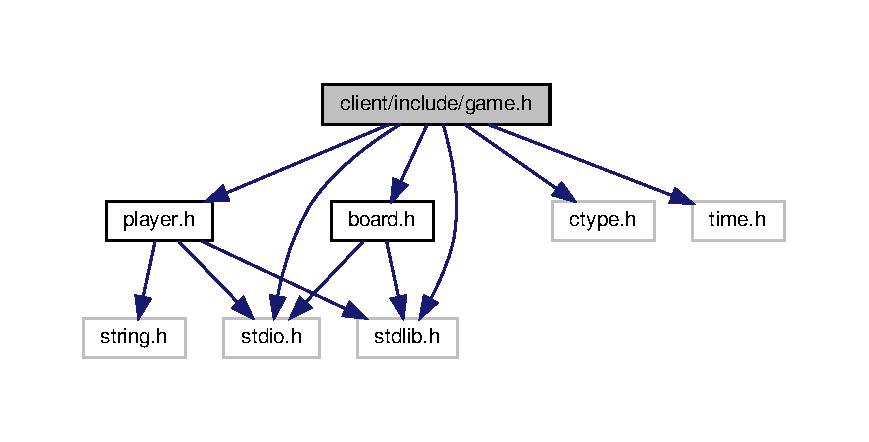
\includegraphics[width=350pt]{game_8h__incl}
\end{center}
\end{figure}
\subsection*{Funções}
\begin{DoxyCompactItemize}
\item 
void \hyperlink{game_8h_a5a57193f6315bcd5fea0e885f0bf6db1}{Print\+Score} (int player1\+Wins, int player2\+Wins, int draws, char $\ast$player1\+Name, char $\ast$player2\+Name)
\begin{DoxyCompactList}\small\item\em Mostrar a pontuação. \end{DoxyCompactList}\item 
void \hyperlink{game_8h_a89454db40f4a9bfe3fb5fc79ce8bc195}{Print\+Winner} (char $\ast$player\+Character, char $\ast$player1\+Name, char $\ast$player2\+Name, int check)
\begin{DoxyCompactList}\small\item\em Mostrar a nome do vencedor. \end{DoxyCompactList}\item 
void \hyperlink{game_8h_ae80136af61d48d4dab91ce44f35f2227}{Play\+Again} (int $\ast$new\+Game)
\begin{DoxyCompactList}\small\item\em Verificar nova partida. \end{DoxyCompactList}\item 
void \hyperlink{game_8h_aba7968c984d7d14474110db10edbe709}{Start\+Game} (int number\+Of\+Players)
\begin{DoxyCompactList}\small\item\em Começar uma partida. \end{DoxyCompactList}\item 
int \hyperlink{game_8h_ade84e17876e747904e3cc149c9d9d18a}{A\+I\+Play} (char game\+Board\mbox{[}9\mbox{]}, int $\ast$chosen\+Number)
\begin{DoxyCompactList}\small\item\em Jogada do computador. \end{DoxyCompactList}\item 
void \hyperlink{game_8h_a8c0cdcbaba5c3fc48e068d3969d264ad}{Player\+Start} (char $\ast$player\+Character, int $\ast$player\+Turn, int number\+Of\+Players, char $\ast$player1\+Name, char $\ast$player2\+Name)
\begin{DoxyCompactList}\small\item\em Definir primeiro jogador. \end{DoxyCompactList}\item 
void \hyperlink{game_8h_ac930428cd81e07f378593efa99b169e9}{Update\+Scores} (int check, char $\ast$player\+Character, int $\ast$player1\+Wins, int $\ast$player2\+Wins, int $\ast$draws, char game\+Board\mbox{[}9\mbox{]})
\begin{DoxyCompactList}\small\item\em Atualiza o marcador de pontos. \end{DoxyCompactList}\item 
void \hyperlink{game_8h_a5b51b82ff890b5f0c120cf42b1c5b04b}{Play\+Game} (char $\ast$player1\+Name, char $\ast$player2\+Name, int number\+Of\+Players)
\begin{DoxyCompactList}\small\item\em Implementa o jogo e suas funções. \end{DoxyCompactList}\end{DoxyCompactItemize}


\subsection{Descrição Detalhada}
Arquivo contendo as estruturas e cabeçalhos de funções do jogo. 

\begin{DoxyAuthor}{Autor}
Vitor Correa da Silva 
\end{DoxyAuthor}
\begin{DoxyDate}{Data}
29 May 2020
\end{DoxyDate}
Esse arquivo contém as definições das funções que são implementadas em game.\+c. Essas funções tem como objetivo implementar o jogo tic-\/tac-\/toe (jogo da velha). 

\subsection{Funções}
\mbox{\Hypertarget{game_8h_ade84e17876e747904e3cc149c9d9d18a}\label{game_8h_ade84e17876e747904e3cc149c9d9d18a}} 
\index{game.\+h@{game.\+h}!A\+I\+Play@{A\+I\+Play}}
\index{A\+I\+Play@{A\+I\+Play}!game.\+h@{game.\+h}}
\subsubsection{\texorpdfstring{A\+I\+Play()}{AIPlay()}}
{\footnotesize\ttfamily int A\+I\+Play (\begin{DoxyParamCaption}\item[{char}]{game\+Board\mbox{[}9\mbox{]},  }\item[{int $\ast$}]{chosen\+Number }\end{DoxyParamCaption})}



Jogada do computador. 

Implementa e simula a jogada do computador. Só é utilizada esta função quando apenas um jogador esta na partida.


\begin{DoxyParams}{Parâmetros}
{\em game\+Board} & Array de 9 posições que guarda as informações do tabuleiro \\
\hline
{\em chosen\+Number} & Valor da possivel jogada \\
\hline
\end{DoxyParams}
\begin{DoxyReturn}{Retorna}
{\ttfamily int} Valor escolhido pelo jogador 
\end{DoxyReturn}
\mbox{\Hypertarget{game_8h_ae80136af61d48d4dab91ce44f35f2227}\label{game_8h_ae80136af61d48d4dab91ce44f35f2227}} 
\index{game.\+h@{game.\+h}!Play\+Again@{Play\+Again}}
\index{Play\+Again@{Play\+Again}!game.\+h@{game.\+h}}
\subsubsection{\texorpdfstring{Play\+Again()}{PlayAgain()}}
{\footnotesize\ttfamily void Play\+Again (\begin{DoxyParamCaption}\item[{int $\ast$}]{new\+Game }\end{DoxyParamCaption})}



Verificar nova partida. 

Verifica se o usuario deseja iniciar uma nova partida, caso nao queira, retorna para o menu.


\begin{DoxyParams}{Parâmetros}
{\em new\+Game} & Verficador de novo jogo. {\bfseries 1} para começar uma nova partida \\
\hline
\end{DoxyParams}
\mbox{\Hypertarget{game_8h_a8c0cdcbaba5c3fc48e068d3969d264ad}\label{game_8h_a8c0cdcbaba5c3fc48e068d3969d264ad}} 
\index{game.\+h@{game.\+h}!Player\+Start@{Player\+Start}}
\index{Player\+Start@{Player\+Start}!game.\+h@{game.\+h}}
\subsubsection{\texorpdfstring{Player\+Start()}{PlayerStart()}}
{\footnotesize\ttfamily void Player\+Start (\begin{DoxyParamCaption}\item[{char $\ast$}]{player\+Character,  }\item[{int $\ast$}]{player\+Turn,  }\item[{int}]{number\+Of\+Players,  }\item[{char $\ast$}]{player1\+Name,  }\item[{char $\ast$}]{player2\+Name }\end{DoxyParamCaption})}



Definir primeiro jogador. 

Define e mostra na tela qual jogador ira comecar a partida.


\begin{DoxyParams}{Parâmetros}
{\em player\+Character} & Caractere do jogador atual \\
\hline
{\em player\+Turn} & Define o turno do jogador \\
\hline
{\em number\+Of\+Players} & Numero de jogadores na partida \\
\hline
{\em player1\+Name} & Nome do jogador numero 1 \\
\hline
{\em player2\+Name} & Nome do jogador numero 2 \\
\hline
\end{DoxyParams}
\mbox{\Hypertarget{game_8h_a5b51b82ff890b5f0c120cf42b1c5b04b}\label{game_8h_a5b51b82ff890b5f0c120cf42b1c5b04b}} 
\index{game.\+h@{game.\+h}!Play\+Game@{Play\+Game}}
\index{Play\+Game@{Play\+Game}!game.\+h@{game.\+h}}
\subsubsection{\texorpdfstring{Play\+Game()}{PlayGame()}}
{\footnotesize\ttfamily void Play\+Game (\begin{DoxyParamCaption}\item[{char $\ast$}]{player1\+Name,  }\item[{char $\ast$}]{player2\+Name,  }\item[{int}]{number\+Of\+Players }\end{DoxyParamCaption})}



Implementa o jogo e suas funções. 

Funcao que controla o fluxo do jogo.


\begin{DoxyParams}{Parâmetros}
{\em player1\+Name} & Nome do jogador numero 1 \\
\hline
{\em player2\+Name} & Nome do jogador numero 2 \\
\hline
{\em number\+Of\+Players} & Numero de jogadores na partida \\
\hline
\end{DoxyParams}
\mbox{\Hypertarget{game_8h_a5a57193f6315bcd5fea0e885f0bf6db1}\label{game_8h_a5a57193f6315bcd5fea0e885f0bf6db1}} 
\index{game.\+h@{game.\+h}!Print\+Score@{Print\+Score}}
\index{Print\+Score@{Print\+Score}!game.\+h@{game.\+h}}
\subsubsection{\texorpdfstring{Print\+Score()}{PrintScore()}}
{\footnotesize\ttfamily void Print\+Score (\begin{DoxyParamCaption}\item[{int}]{player1\+Wins,  }\item[{int}]{player2\+Wins,  }\item[{int}]{draws,  }\item[{char $\ast$}]{player1\+Name,  }\item[{char $\ast$}]{player2\+Name }\end{DoxyParamCaption})}



Mostrar a pontuação. 

Escreve a pontuacao atual dos jogadores na tela.


\begin{DoxyParams}{Parâmetros}
{\em player1\+Wins} & Numero de vitorias do jogador 1 \\
\hline
{\em player2\+Wins} & Numero de vitorias do jogador 2 \\
\hline
{\em draws} & Numero de empates entre os dois jogadores \\
\hline
{\em player1\+Name} & Nome do jogador numero 1 \\
\hline
{\em player2\+Name} & Nome do jogador numero 2 \\
\hline
\end{DoxyParams}
\mbox{\Hypertarget{game_8h_a89454db40f4a9bfe3fb5fc79ce8bc195}\label{game_8h_a89454db40f4a9bfe3fb5fc79ce8bc195}} 
\index{game.\+h@{game.\+h}!Print\+Winner@{Print\+Winner}}
\index{Print\+Winner@{Print\+Winner}!game.\+h@{game.\+h}}
\subsubsection{\texorpdfstring{Print\+Winner()}{PrintWinner()}}
{\footnotesize\ttfamily void Print\+Winner (\begin{DoxyParamCaption}\item[{char $\ast$}]{player\+Character,  }\item[{char $\ast$}]{player1\+Name,  }\item[{char $\ast$}]{player2\+Name,  }\item[{int}]{check }\end{DoxyParamCaption})}



Mostrar a nome do vencedor. 

Escreve na tela o nome do vencedor, se houve algum, ou se houve empate


\begin{DoxyParams}{Parâmetros}
{\em player\+Character} & Caractere do joogador. Pode ser {\bfseries X} ou {\bfseries O} \\
\hline
{\em player1\+Name} & Nome do jogador 1 \\
\hline
{\em player2\+Name} & Nome do jogador 2 \\
\hline
{\em check} & Verificador de vitoria ou empate. {\bfseries 1} se houver vencedo ou {\bfseries 2} se for um empate \\
\hline
\end{DoxyParams}
\mbox{\Hypertarget{game_8h_aba7968c984d7d14474110db10edbe709}\label{game_8h_aba7968c984d7d14474110db10edbe709}} 
\index{game.\+h@{game.\+h}!Start\+Game@{Start\+Game}}
\index{Start\+Game@{Start\+Game}!game.\+h@{game.\+h}}
\subsubsection{\texorpdfstring{Start\+Game()}{StartGame()}}
{\footnotesize\ttfamily void Start\+Game (\begin{DoxyParamCaption}\item[{int}]{number\+Of\+Players }\end{DoxyParamCaption})}



Começar uma partida. 

Define do nome dos jogadores e chama a funcao de inicio do jogo.


\begin{DoxyParams}{Parâmetros}
{\em number\+Of\+Players} & Numero de jogadores na partida \\
\hline
\end{DoxyParams}
\mbox{\Hypertarget{game_8h_ac930428cd81e07f378593efa99b169e9}\label{game_8h_ac930428cd81e07f378593efa99b169e9}} 
\index{game.\+h@{game.\+h}!Update\+Scores@{Update\+Scores}}
\index{Update\+Scores@{Update\+Scores}!game.\+h@{game.\+h}}
\subsubsection{\texorpdfstring{Update\+Scores()}{UpdateScores()}}
{\footnotesize\ttfamily void Update\+Scores (\begin{DoxyParamCaption}\item[{int}]{check,  }\item[{char $\ast$}]{player\+Character,  }\item[{int $\ast$}]{player1\+Wins,  }\item[{int $\ast$}]{player2\+Wins,  }\item[{int $\ast$}]{draws,  }\item[{char}]{game\+Board\mbox{[}9\mbox{]} }\end{DoxyParamCaption})}



Atualiza o marcador de pontos. 

Atualiza os placares e altera o valor da variavel que controla o loop (win).


\begin{DoxyParams}{Parâmetros}
{\em check} & Verificador de vitoria ou empate. {\bfseries 1} se houver vencedo ou {\bfseries 2} se for um empate \\
\hline
{\em player\+Character} & Caractere do joogador. Pode ser {\bfseries X} ou {\bfseries O} \\
\hline
{\em player1\+Wins} & Numero de vitorias do jogador 1 \\
\hline
{\em player2\+Wins} & Numero de vitorias do jogador 2 \\
\hline
{\em draws} & Numero de empates entre os dois jogadores \\
\hline
{\em game\+Board} & Array de 9 posições que guarda as informações do tabuleiro \\
\hline
\end{DoxyParams}

\hypertarget{menu_8h}{}\section{Referência do Arquivo client/include/menu.h}
\label{menu_8h}\index{client/include/menu.\+h@{client/include/menu.\+h}}


Arquivo contendo as estruturas e cabeçalhos de funções do menu.  


{\ttfamily \#include $<$stdio.\+h$>$}\newline
{\ttfamily \#include $<$stdlib.\+h$>$}\newline
Gráfico de dependência de inclusões para menu.\+h\+:
\nopagebreak
\begin{figure}[H]
\begin{center}
\leavevmode
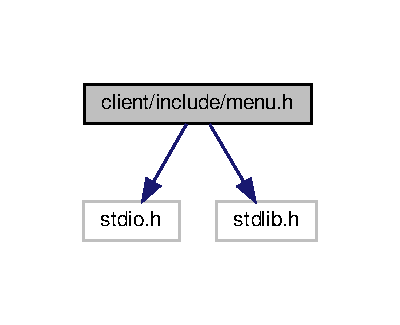
\includegraphics[width=192pt]{menu_8h__incl}
\end{center}
\end{figure}
Este grafo mostra quais arquivos estão direta ou indiretamente relacionados com este arquivo\+:
\nopagebreak
\begin{figure}[H]
\begin{center}
\leavevmode
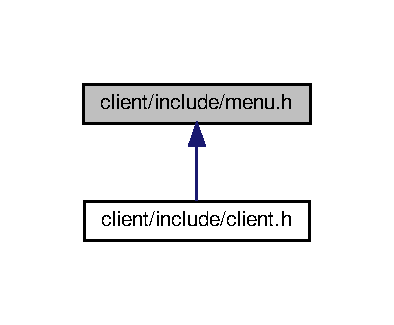
\includegraphics[width=189pt]{menu_8h__dep__incl}
\end{center}
\end{figure}
\subsection*{Funções}
\begin{DoxyCompactItemize}
\item 
void \hyperlink{menu_8h_a320076d5ec51536af9676b6ae5d38e7b}{Show\+Menu} ()
\begin{DoxyCompactList}\small\item\em Mostra o menu. \end{DoxyCompactList}\item 
void \hyperlink{menu_8h_ac7e4de9786226cbd71e4f86de310a3d7}{Menu\+Choice} (int choice, int $\ast$number\+Of\+Players)
\begin{DoxyCompactList}\small\item\em Chama a função escolhida pelo jogador. \end{DoxyCompactList}\end{DoxyCompactItemize}


\subsection{Descrição Detalhada}
Arquivo contendo as estruturas e cabeçalhos de funções do menu. 

\begin{DoxyAuthor}{Autor}
Vitor Correa da Silva 
\end{DoxyAuthor}
\begin{DoxyDate}{Data}
29 May 2020
\end{DoxyDate}
Esse arquivo contém as definições das funções que são implementadas em menu.\+c. Essas funções tem como objetivo implementar um menu interativo. 

\subsection{Funções}
\mbox{\Hypertarget{menu_8h_ac7e4de9786226cbd71e4f86de310a3d7}\label{menu_8h_ac7e4de9786226cbd71e4f86de310a3d7}} 
\index{menu.\+h@{menu.\+h}!Menu\+Choice@{Menu\+Choice}}
\index{Menu\+Choice@{Menu\+Choice}!menu.\+h@{menu.\+h}}
\subsubsection{\texorpdfstring{Menu\+Choice()}{MenuChoice()}}
{\footnotesize\ttfamily void Menu\+Choice (\begin{DoxyParamCaption}\item[{int}]{choice,  }\item[{int $\ast$}]{number\+Of\+Players }\end{DoxyParamCaption})}



Chama a função escolhida pelo jogador. 

Espera um {\bfseries int} para definir a escolha do jogador e depois faz a chamada da função escolhida.


\begin{DoxyParams}{Parâmetros}
{\em choice} & Escolha do jogador \\
\hline
{\em number\+Of\+Players} & Numero de jogadores \\
\hline
\end{DoxyParams}
\mbox{\Hypertarget{menu_8h_a320076d5ec51536af9676b6ae5d38e7b}\label{menu_8h_a320076d5ec51536af9676b6ae5d38e7b}} 
\index{menu.\+h@{menu.\+h}!Show\+Menu@{Show\+Menu}}
\index{Show\+Menu@{Show\+Menu}!menu.\+h@{menu.\+h}}
\subsubsection{\texorpdfstring{Show\+Menu()}{ShowMenu()}}
{\footnotesize\ttfamily void Show\+Menu (\begin{DoxyParamCaption}{ }\end{DoxyParamCaption})}



Mostra o menu. 

Implemtação do texto que é mostrado no menu 
\hypertarget{player_8h}{}\section{Referência do Arquivo client/include/player.h}
\label{player_8h}\index{client/include/player.\+h@{client/include/player.\+h}}


Arquivo contendo cabeçalhos de funções que implementam as funções do player.  


{\ttfamily \#include $<$stdio.\+h$>$}\newline
{\ttfamily \#include $<$stdlib.\+h$>$}\newline
{\ttfamily \#include $<$string.\+h$>$}\newline
Gráfico de dependência de inclusões para player.\+h\+:
\nopagebreak
\begin{figure}[H]
\begin{center}
\leavevmode
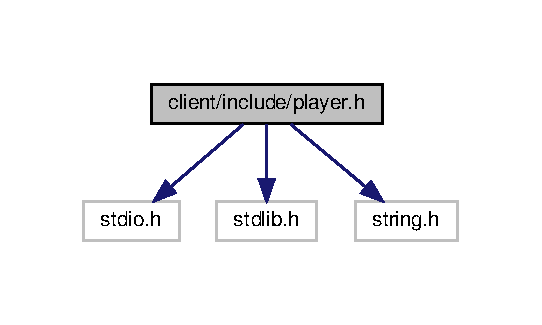
\includegraphics[width=260pt]{player_8h__incl}
\end{center}
\end{figure}
Este grafo mostra quais arquivos estão direta ou indiretamente relacionados com este arquivo\+:
\nopagebreak
\begin{figure}[H]
\begin{center}
\leavevmode
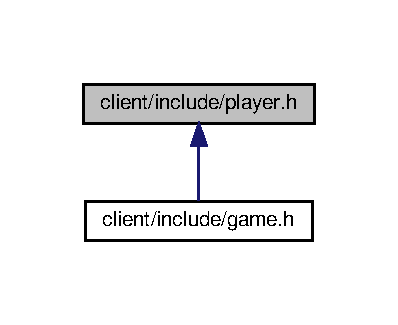
\includegraphics[width=191pt]{player_8h__dep__incl}
\end{center}
\end{figure}
\subsection*{Funções}
\begin{DoxyCompactItemize}
\item 
void \hyperlink{player_8h_a7ee9285c4f799709a278367aa89c3ddd}{Change\+Player} (char $\ast$player\+Character)
\begin{DoxyCompactList}\small\item\em Muda o caractere do jogador atual. \end{DoxyCompactList}\item 
int \hyperlink{player_8h_ac6ec12daed56156840312167f3b666ec}{Get\+Number\+Of\+Players} ()
\begin{DoxyCompactList}\small\item\em Retorna o numero de jogadores. \end{DoxyCompactList}\item 
char $\ast$ \hyperlink{player_8h_a44cb69b8503cd66d7847cc15965d7308}{Get\+Player\+Name} (int player\+Number)
\begin{DoxyCompactList}\small\item\em Define o nome do jogador. \end{DoxyCompactList}\end{DoxyCompactItemize}


\subsection{Descrição Detalhada}
Arquivo contendo cabeçalhos de funções que implementam as funções do player. 

\begin{DoxyAuthor}{Autor}
Vitor Correa da Silva 
\end{DoxyAuthor}
\begin{DoxyDate}{Data}
29 May 2020
\end{DoxyDate}
Esse arquivo contém as definições das funções que são implementadas em player.\+c. Essas funções tem como objetivo implementar as operações de escolha de caracter para os jogadores, escolha do numero de jogadores e define o nome do jogador. 

\subsection{Funções}
\mbox{\Hypertarget{player_8h_a7ee9285c4f799709a278367aa89c3ddd}\label{player_8h_a7ee9285c4f799709a278367aa89c3ddd}} 
\index{player.\+h@{player.\+h}!Change\+Player@{Change\+Player}}
\index{Change\+Player@{Change\+Player}!player.\+h@{player.\+h}}
\subsubsection{\texorpdfstring{Change\+Player()}{ChangePlayer()}}
{\footnotesize\ttfamily void Change\+Player (\begin{DoxyParamCaption}\item[{char $\ast$}]{player\+Character }\end{DoxyParamCaption})}



Muda o caractere do jogador atual. 

Decide o caractere a ser usado pelo jogador.


\begin{DoxyParams}{Parâmetros}
{\em player\+Character} & Ponteiro que guarda a informação de caractere do jogador. \\
\hline
\end{DoxyParams}
\mbox{\Hypertarget{player_8h_ac6ec12daed56156840312167f3b666ec}\label{player_8h_ac6ec12daed56156840312167f3b666ec}} 
\index{player.\+h@{player.\+h}!Get\+Number\+Of\+Players@{Get\+Number\+Of\+Players}}
\index{Get\+Number\+Of\+Players@{Get\+Number\+Of\+Players}!player.\+h@{player.\+h}}
\subsubsection{\texorpdfstring{Get\+Number\+Of\+Players()}{GetNumberOfPlayers()}}
{\footnotesize\ttfamily int Get\+Number\+Of\+Players (\begin{DoxyParamCaption}{ }\end{DoxyParamCaption})}



Retorna o numero de jogadores. 

Implementa a escolha do numero de jogadores 1 ou 2.

\begin{DoxyReturn}{Retorna}
{\ttfamily int} contendo o numero de jogadores da partida. Retorna {\bfseries 1} ou {\bfseries 2} jogadores. 
\end{DoxyReturn}
\mbox{\Hypertarget{player_8h_a44cb69b8503cd66d7847cc15965d7308}\label{player_8h_a44cb69b8503cd66d7847cc15965d7308}} 
\index{player.\+h@{player.\+h}!Get\+Player\+Name@{Get\+Player\+Name}}
\index{Get\+Player\+Name@{Get\+Player\+Name}!player.\+h@{player.\+h}}
\subsubsection{\texorpdfstring{Get\+Player\+Name()}{GetPlayerName()}}
{\footnotesize\ttfamily char$\ast$ Get\+Player\+Name (\begin{DoxyParamCaption}\item[{int}]{player\+Number }\end{DoxyParamCaption})}



Define o nome do jogador. 

Define o nome do jogador que é retornornado como ponteiro {\ttfamily $\ast$char} 


\begin{DoxyParams}{Parâmetros}
{\em player\+Number} & Contem o numero do jogador que deve alterar o nome. {\bfseries 0} para computador {\bfseries 1} ou {\bfseries 2} para os jogadores. \\
\hline
\end{DoxyParams}
\begin{DoxyReturn}{Retorna}
{\ttfamily $\ast$char} contendo o nome do jogador. 
\end{DoxyReturn}

\hypertarget{client__thread_8h}{}\section{Referência do Arquivo server/include/client\+\_\+thread.h}
\label{client__thread_8h}\index{server/include/client\+\_\+thread.\+h@{server/include/client\+\_\+thread.\+h}}


Arquivo contendo cabeçalhos de funções que implementam as interações do servidor com os clientes conectados.  


Este grafo mostra quais arquivos estão direta ou indiretamente relacionados com este arquivo\+:
\nopagebreak
\begin{figure}[H]
\begin{center}
\leavevmode
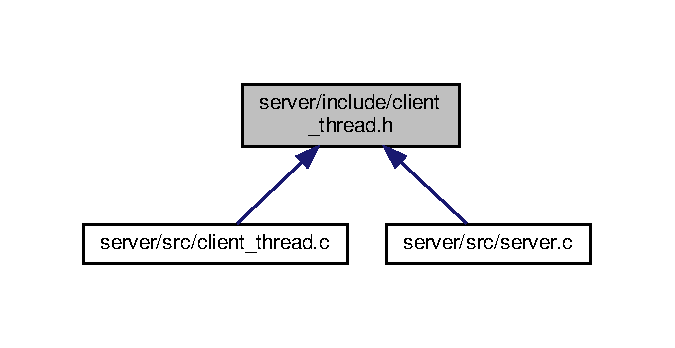
\includegraphics[width=324pt]{client__thread_8h__dep__incl}
\end{center}
\end{figure}
\subsection*{Definições e Macros}
\begin{DoxyCompactItemize}
\item 
\mbox{\Hypertarget{client__thread_8h_ac99ae6be8f999a0293faad128a6ab850}\label{client__thread_8h_ac99ae6be8f999a0293faad128a6ab850}} 
\#define {\bfseries T\+A\+M\+\_\+\+J\+O\+G\+A\+DA}~1089
\end{DoxyCompactItemize}
\subsection*{Funções}
\begin{DoxyCompactItemize}
\item 
int \hyperlink{client__thread_8h_aa54065880f42cda8bec65d90455adda0}{init\+\_\+shared\+\_\+variables} (void)
\begin{DoxyCompactList}\small\item\em Inicializa as variáveis compartilhadas. \end{DoxyCompactList}\item 
void $\ast$ \hyperlink{client__thread_8h_a86e63437485b25c41bbb1f60486084e9}{client\+\_\+connection\+\_\+thread} (void $\ast$client\+\_\+address)
\begin{DoxyCompactList}\small\item\em Thread de conexão dedicada a um cliente. \end{DoxyCompactList}\item 
void \hyperlink{client__thread_8h_ac6bc41cb445fb65d6e0f6d5740789cb4}{start\+\_\+remote\+\_\+tictactoe\+\_\+game} (int socket, \hyperlink{server_8h_a9c8780378078e51e7c9041cbac392db9}{Player} p, unsigned short game\+\_\+id)
\begin{DoxyCompactList}\small\item\em Inicia uma partida de tic-\/tac-\/toe com o jogador indicado. \end{DoxyCompactList}\item 
int \hyperlink{client__thread_8h_a0c2a40bfec08e5623244ec2377b5cfff}{search\+\_\+for\+\_\+available\+\_\+game} (void)
\begin{DoxyCompactList}\small\item\em Procura por um jogo com vagas abertas. \end{DoxyCompactList}\item 
int \hyperlink{client__thread_8h_a28fe4040784cc676e1d0a757cdb02628}{insert\+\_\+player\+\_\+in\+\_\+game} (\hyperlink{server_8h_a9c8780378078e51e7c9041cbac392db9}{Player} p, int game\+\_\+id)
\begin{DoxyCompactList}\small\item\em Insere um jogador em uma partida. \end{DoxyCompactList}\item 
void \hyperlink{client__thread_8h_ac75eae4133f6e5bde445e1380ee07d58}{wait\+\_\+all\+\_\+players\+\_\+to\+\_\+connect} (int game\+\_\+id)
\begin{DoxyCompactList}\small\item\em Espera até que todos os jogadores se conectem em uma partida. \end{DoxyCompactList}\item 
void \hyperlink{client__thread_8h_a8adfa2e21b4f3b6c6ed0eed53b7b6c8c}{write\+\_\+in\+\_\+file\+\_\+ranking} (char $\ast$msg)
\begin{DoxyCompactList}\small\item\em Cria um arquivo com o nome dos vencedores. \end{DoxyCompactList}\item 
void \hyperlink{client__thread_8h_a42a0849dd88c8efd0747a304aa5ecea5}{leave\+\_\+game} (int game\+\_\+id)
\begin{DoxyCompactList}\small\item\em Abandona uma partida. \end{DoxyCompactList}\end{DoxyCompactItemize}


\subsection{Descrição Detalhada}
Arquivo contendo cabeçalhos de funções que implementam as interações do servidor com os clientes conectados. 

\begin{DoxyAuthor}{Autor}
Vitor Correa da Silva 
\end{DoxyAuthor}
\begin{DoxyDate}{Data}
29 May 2020
\end{DoxyDate}
Esse arquivo contém as definições das funções que são implementadas em \hyperlink{client__thread_8c}{client\+\_\+thread.\+c}. Essas funções tem como objetivo implementar o funcionamento da troca de mensagens entre servidor e clientes quando estes já estão conectados. 

\subsection{Funções}
\mbox{\Hypertarget{client__thread_8h_a86e63437485b25c41bbb1f60486084e9}\label{client__thread_8h_a86e63437485b25c41bbb1f60486084e9}} 
\index{client\+\_\+thread.\+h@{client\+\_\+thread.\+h}!client\+\_\+connection\+\_\+thread@{client\+\_\+connection\+\_\+thread}}
\index{client\+\_\+connection\+\_\+thread@{client\+\_\+connection\+\_\+thread}!client\+\_\+thread.\+h@{client\+\_\+thread.\+h}}
\subsubsection{\texorpdfstring{client\+\_\+connection\+\_\+thread()}{client\_connection\_thread()}}
{\footnotesize\ttfamily void$\ast$ client\+\_\+connection\+\_\+thread (\begin{DoxyParamCaption}\item[{void $\ast$}]{client\+\_\+address }\end{DoxyParamCaption})}



Thread de conexão dedicada a um cliente. 

Essa função é chamada em forma de thread sempre que um usuário realiza login no servidor, recebendo o endereço {\ttfamily client\+\_\+address} do client como parâmetro. Essa função faz as seguintes ações\+:
\begin{DoxyItemize}
\item Realizar a abertura de um socket dedicado para o cliente, e envia o endereço do socket para o cliente.
\item Receber e armazenar o nome do cliente conectado.
\item Chamar a função {\ttfamily search\+\_\+for\+\_\+available\+\_\+game} para encontrar uma partida para esse jogador.
\item Chamar a função {\ttfamily insert\+\_\+player\+\_\+in\+\_\+game} para inserir esse jogador na partida encontrada.
\item Caso o jogador for o primeiro a se conectar a partida, espera até que o segundo se conecte chamando a função {\ttfamily wait\+\_\+all\+\_\+players\+\_\+to\+\_\+connect}.
\item Caso o jogador for o segundo a se conectar na partida, realiza o sorteio de quem é o primeiro a jogar.
\item Avisa os jogadores se são os primeiros ou segundos a jogar.
\item Inicia a partida dos jogadores com a função {\ttfamily start\+\_\+remote\+\_\+tictactoe\+\_\+game}.
\item Fecha os socket abertos, ao fim da partida.
\end{DoxyItemize}


\begin{DoxyParams}{Parâmetros}
{\em client\+\_\+address} & Ponteiro para o endereço do cliente conectado. \\
\hline
\end{DoxyParams}
\begin{DoxyReturn}{Retorna}
Não há retorno. 
\end{DoxyReturn}
\mbox{\Hypertarget{client__thread_8h_aa54065880f42cda8bec65d90455adda0}\label{client__thread_8h_aa54065880f42cda8bec65d90455adda0}} 
\index{client\+\_\+thread.\+h@{client\+\_\+thread.\+h}!init\+\_\+shared\+\_\+variables@{init\+\_\+shared\+\_\+variables}}
\index{init\+\_\+shared\+\_\+variables@{init\+\_\+shared\+\_\+variables}!client\+\_\+thread.\+h@{client\+\_\+thread.\+h}}
\subsubsection{\texorpdfstring{init\+\_\+shared\+\_\+variables()}{init\_shared\_variables()}}
{\footnotesize\ttfamily int init\+\_\+shared\+\_\+variables (\begin{DoxyParamCaption}\item[{void}]{ }\end{DoxyParamCaption})}



Inicializa as variáveis compartilhadas. 

Essa função inicializa as variáveis que são compartilhadas entre as threads de conexão com os clientes. Inicializa os seguintes recursos\+:
\begin{DoxyItemize}
\item pthread\+\_\+mutex\+\_\+t lock
\item Game tictactoe\mbox{[}N\+R\+O\+\_\+\+P\+A\+R\+T\+I\+D\+A\+S\+\_\+\+S\+I\+M\+U\+L\+T\+A\+N\+E\+AS\mbox{]}
\end{DoxyItemize}

{\ttfamily lock} é o mutex utilizado para controlar o acesso à variável {\ttfamily tictactoe} , realizando a exclusão mútua de acesso à mesma. Fazendo com que não mais que uma thread possa adentrar uma região de código trancada por essa variável.

{\ttfamily tictactoe} é um array que contém todos os jogos do servidor, e é utilizado pelas várias threads de clientes para ler as informações da partida, entrar em partidas, etc.

\begin{DoxyReturn}{Retorna}
resultado da inicialização\+: 0 em caso de sucesso e 1 em caso de erro. 
\end{DoxyReturn}
\mbox{\Hypertarget{client__thread_8h_a28fe4040784cc676e1d0a757cdb02628}\label{client__thread_8h_a28fe4040784cc676e1d0a757cdb02628}} 
\index{client\+\_\+thread.\+h@{client\+\_\+thread.\+h}!insert\+\_\+player\+\_\+in\+\_\+game@{insert\+\_\+player\+\_\+in\+\_\+game}}
\index{insert\+\_\+player\+\_\+in\+\_\+game@{insert\+\_\+player\+\_\+in\+\_\+game}!client\+\_\+thread.\+h@{client\+\_\+thread.\+h}}
\subsubsection{\texorpdfstring{insert\+\_\+player\+\_\+in\+\_\+game()}{insert\_player\_in\_game()}}
{\footnotesize\ttfamily int insert\+\_\+player\+\_\+in\+\_\+game (\begin{DoxyParamCaption}\item[{\hyperlink{server_8h_a9c8780378078e51e7c9041cbac392db9}{Player}}]{p,  }\item[{int}]{game\+\_\+id }\end{DoxyParamCaption})}



Insere um jogador em uma partida. 

Insere o jogador {\ttfamily p} dentro da partida {\ttfamily game\+\_\+id}, na primeira ou segunda posição.


\begin{DoxyParams}{Parâmetros}
{\em p} & Jogador que será inserido. \\
\hline
{\em game\+\_\+id} & Partida que terá um jogador inserido. \\
\hline
\end{DoxyParams}
\begin{DoxyReturn}{Retorna}
{\ttfamily int} id do jogador dentro dessa partida, sendo 0 ou 1
\end{DoxyReturn}
{\bfseries Exemplo de uso\+:} 
\begin{DoxyCode}
\hyperlink{structplayer}{Player} p;
\textcolor{keywordtype}{int} game\_id;

game\_id = \hyperlink{client__thread_8h_a0c2a40bfec08e5623244ec2377b5cfff}{search\_for\_available\_game}();
\textcolor{keywordflow}{if} (game\_id == -1)
\{
    printf(\textcolor{stringliteral}{"Não há partidas com vagas.\(\backslash\)n"});
\}
\textcolor{keywordflow}{else}
\{
    p.\hyperlink{structplayer_a0e6fb0e744015cdf9f4dd12164a1dbaa}{id} = \hyperlink{client__thread_8h_a28fe4040784cc676e1d0a757cdb02628}{insert\_player\_in\_game}(p, game\_id);
\}
\end{DoxyCode}


\begin{DoxyWarning}{Aviso}
É recomendável que essa função seja chamada dentro do bloqueio do mutex. Para impedir que mais de 2 jogadores tentem entrar na mesma partida ao mesmo tempo e quebre o limite de jogadores por partida. 
\end{DoxyWarning}
\mbox{\Hypertarget{client__thread_8h_a42a0849dd88c8efd0747a304aa5ecea5}\label{client__thread_8h_a42a0849dd88c8efd0747a304aa5ecea5}} 
\index{client\+\_\+thread.\+h@{client\+\_\+thread.\+h}!leave\+\_\+game@{leave\+\_\+game}}
\index{leave\+\_\+game@{leave\+\_\+game}!client\+\_\+thread.\+h@{client\+\_\+thread.\+h}}
\subsubsection{\texorpdfstring{leave\+\_\+game()}{leave\_game()}}
{\footnotesize\ttfamily void leave\+\_\+game (\begin{DoxyParamCaption}\item[{int}]{game\+\_\+id }\end{DoxyParamCaption})}



Abandona uma partida. 

Decrementa em um o número de jogadores de uma partida;


\begin{DoxyParams}{Parâmetros}
{\em game\+\_\+id} & id da partida. \\
\hline
\end{DoxyParams}
\begin{DoxyReturn}{Retorna}
Não há retorno. 
\end{DoxyReturn}
\mbox{\Hypertarget{client__thread_8h_a0c2a40bfec08e5623244ec2377b5cfff}\label{client__thread_8h_a0c2a40bfec08e5623244ec2377b5cfff}} 
\index{client\+\_\+thread.\+h@{client\+\_\+thread.\+h}!search\+\_\+for\+\_\+available\+\_\+game@{search\+\_\+for\+\_\+available\+\_\+game}}
\index{search\+\_\+for\+\_\+available\+\_\+game@{search\+\_\+for\+\_\+available\+\_\+game}!client\+\_\+thread.\+h@{client\+\_\+thread.\+h}}
\subsubsection{\texorpdfstring{search\+\_\+for\+\_\+available\+\_\+game()}{search\_for\_available\_game()}}
{\footnotesize\ttfamily int search\+\_\+for\+\_\+available\+\_\+game (\begin{DoxyParamCaption}\item[{void}]{ }\end{DoxyParamCaption})}



Procura por um jogo com vagas abertas. 

Faz a busca por uma partida com vagas abertas no servidor, o procedimento de busca é o seguinte\+:
\begin{DoxyItemize}
\item Se houver uma partida com um player esperando um oponente, dá preferência a essa partida.
\item Se não houver partida com um player esperando, procura pela primeira partida com duas vagas abertas.
\item Se todas as partidas estiverem cheias, retorna {\bfseries -\/1} , indicando que não há vagas.
\end{DoxyItemize}

\begin{DoxyReturn}{Retorna}
Id da partida encontrada.
\end{DoxyReturn}
{\bfseries Exemplo de uso\+:} 
\begin{DoxyCode}
\hyperlink{structplayer}{Player} p;
\textcolor{keywordtype}{int} game\_id;

game\_id = \hyperlink{client__thread_8h_a0c2a40bfec08e5623244ec2377b5cfff}{search\_for\_available\_game}();
\textcolor{keywordflow}{if} (game\_id == -1)
\{
    printf(\textcolor{stringliteral}{"Não há partidas com vagas.\(\backslash\)n"});
\}
\textcolor{keywordflow}{else}
\{
    p.\hyperlink{structplayer_a0e6fb0e744015cdf9f4dd12164a1dbaa}{id} = \hyperlink{client__thread_8h_a28fe4040784cc676e1d0a757cdb02628}{insert\_player\_in\_game}(p, game\_id);
\}
\end{DoxyCode}


\begin{DoxyWarning}{Aviso}
É recomendável que essa partida seja chamada dentro do bloqueio do mutex, para evitar que as informações das partidas sejam alteradas durante a busca. 
\end{DoxyWarning}
\mbox{\Hypertarget{client__thread_8h_ac6bc41cb445fb65d6e0f6d5740789cb4}\label{client__thread_8h_ac6bc41cb445fb65d6e0f6d5740789cb4}} 
\index{client\+\_\+thread.\+h@{client\+\_\+thread.\+h}!start\+\_\+remote\+\_\+tictactoe\+\_\+game@{start\+\_\+remote\+\_\+tictactoe\+\_\+game}}
\index{start\+\_\+remote\+\_\+tictactoe\+\_\+game@{start\+\_\+remote\+\_\+tictactoe\+\_\+game}!client\+\_\+thread.\+h@{client\+\_\+thread.\+h}}
\subsubsection{\texorpdfstring{start\+\_\+remote\+\_\+tictactoe\+\_\+game()}{start\_remote\_tictactoe\_game()}}
{\footnotesize\ttfamily void start\+\_\+remote\+\_\+tictactoe\+\_\+game (\begin{DoxyParamCaption}\item[{int}]{socket,  }\item[{\hyperlink{server_8h_a9c8780378078e51e7c9041cbac392db9}{Player}}]{p,  }\item[{unsigned short}]{game\+\_\+id }\end{DoxyParamCaption})}



Inicia uma partida de tic-\/tac-\/toe com o jogador indicado. 

Essa função implementa a troca de mensagens de um jogador com a partida, e deve ser chamada pelos dois jogadores. Um é o jogador que foi sorteado para começar, o outro para ser o segundo a jogar. A razão para isso é que a conexão dos dois clientes é tratada independentemente em duas threads, e a função é chamada quase que simultaneamente pelas duas threads ao fim da função {\ttfamily wait\+\_\+all\+\_\+players\+\_\+to\+\_\+connect}.

Quando a partida acaba, é chamada a função {\ttfamily leave\+\_\+game}.


\begin{DoxyParams}{Parâmetros}
{\em socket} & Socket que o servidor esperará por mensagens desse jogador e enviará jogadas a seu oponente. \\
\hline
{\em p} & Jogador que participará da partida. \\
\hline
{\em game\+\_\+id} & id da partida que está iniciando. \\
\hline
\end{DoxyParams}
\begin{DoxyReturn}{Retorna}
Não há retorno. 
\end{DoxyReturn}
\mbox{\Hypertarget{client__thread_8h_ac75eae4133f6e5bde445e1380ee07d58}\label{client__thread_8h_ac75eae4133f6e5bde445e1380ee07d58}} 
\index{client\+\_\+thread.\+h@{client\+\_\+thread.\+h}!wait\+\_\+all\+\_\+players\+\_\+to\+\_\+connect@{wait\+\_\+all\+\_\+players\+\_\+to\+\_\+connect}}
\index{wait\+\_\+all\+\_\+players\+\_\+to\+\_\+connect@{wait\+\_\+all\+\_\+players\+\_\+to\+\_\+connect}!client\+\_\+thread.\+h@{client\+\_\+thread.\+h}}
\subsubsection{\texorpdfstring{wait\+\_\+all\+\_\+players\+\_\+to\+\_\+connect()}{wait\_all\_players\_to\_connect()}}
{\footnotesize\ttfamily void wait\+\_\+all\+\_\+players\+\_\+to\+\_\+connect (\begin{DoxyParamCaption}\item[{int}]{game\+\_\+id }\end{DoxyParamCaption})}



Espera até que todos os jogadores se conectem em uma partida. 

{\bfseries Bloqueia} a execução do programa até que a partida de id {\ttfamily game\+\_\+id} esteja cheia.


\begin{DoxyParams}{Parâmetros}
{\em game\+\_\+id} & id da partida \\
\hline
\end{DoxyParams}
\begin{DoxyReturn}{Retorna}
Não há retorno.
\end{DoxyReturn}
\begin{DoxyWarning}{Aviso}
Se essa função for chamada dentro do bloqueio do mutex, ela nunca será finalizada. 
\end{DoxyWarning}
\mbox{\Hypertarget{client__thread_8h_a8adfa2e21b4f3b6c6ed0eed53b7b6c8c}\label{client__thread_8h_a8adfa2e21b4f3b6c6ed0eed53b7b6c8c}} 
\index{client\+\_\+thread.\+h@{client\+\_\+thread.\+h}!write\+\_\+in\+\_\+file\+\_\+ranking@{write\+\_\+in\+\_\+file\+\_\+ranking}}
\index{write\+\_\+in\+\_\+file\+\_\+ranking@{write\+\_\+in\+\_\+file\+\_\+ranking}!client\+\_\+thread.\+h@{client\+\_\+thread.\+h}}
\subsubsection{\texorpdfstring{write\+\_\+in\+\_\+file\+\_\+ranking()}{write\_in\_file\_ranking()}}
{\footnotesize\ttfamily void write\+\_\+in\+\_\+file\+\_\+ranking (\begin{DoxyParamCaption}\item[{char $\ast$}]{msg }\end{DoxyParamCaption})}



Cria um arquivo com o nome dos vencedores. 

Cria um novo arquivo ou abre um ja existente e escreve o nome do vencedor da partida.


\begin{DoxyParams}{Parâmetros}
{\em msg} & nome do jogador vencedor \\
\hline
\end{DoxyParams}
\begin{DoxyReturn}{Retorna}
Não há retorno. 
\end{DoxyReturn}

\hypertarget{server_8h}{}\section{Referência do Arquivo server/include/server.h}
\label{server_8h}\index{server/include/server.\+h@{server/include/server.\+h}}


Arquivo contendo as estruturas e cabeçalhos de funções do servidor.  


{\ttfamily \#include $<$netinet/in.\+h$>$}\newline
{\ttfamily \#include $<$unistd.\+h$>$}\newline
{\ttfamily \#include $<$stdio.\+h$>$}\newline
{\ttfamily \#include $<$string.\+h$>$}\newline
{\ttfamily \#include $<$stdlib.\+h$>$}\newline
{\ttfamily \#include $<$pthread.\+h$>$}\newline
Gráfico de dependência de inclusões para server.\+h\+:
\nopagebreak
\begin{figure}[H]
\begin{center}
\leavevmode
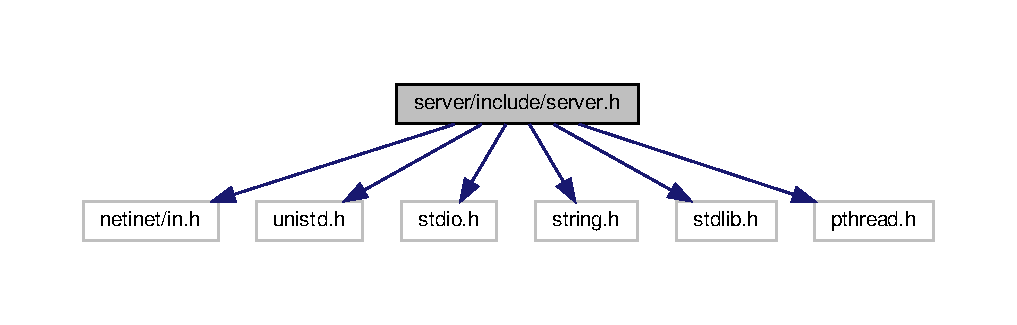
\includegraphics[width=350pt]{server_8h__incl}
\end{center}
\end{figure}
Este grafo mostra quais arquivos estão direta ou indiretamente relacionados com este arquivo\+:
\nopagebreak
\begin{figure}[H]
\begin{center}
\leavevmode
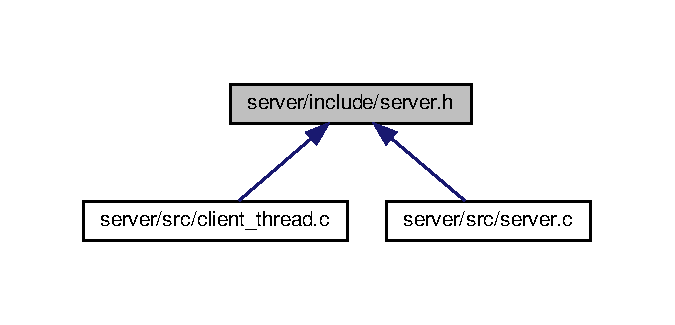
\includegraphics[width=324pt]{server_8h__dep__incl}
\end{center}
\end{figure}
\subsection*{Estruturas de Dados}
\begin{DoxyCompactItemize}
\item 
struct \hyperlink{structreceived__message}{received\+\_\+message}
\item 
struct \hyperlink{structplayer}{player}
\item 
struct \hyperlink{structgame}{game}
\end{DoxyCompactItemize}
\subsection*{Definições e Macros}
\begin{DoxyCompactItemize}
\item 
\mbox{\Hypertarget{server_8h_a4af527b772cacbae6d6a0e48c3dcf53f}\label{server_8h_a4af527b772cacbae6d6a0e48c3dcf53f}} 
\#define {\bfseries T\+A\+M\+\_\+\+M\+SG}~1024
\item 
\mbox{\Hypertarget{server_8h_a06cb24e830bc294c5ec50624f5b6263e}\label{server_8h_a06cb24e830bc294c5ec50624f5b6263e}} 
\#define {\bfseries N\+R\+O\+\_\+\+P\+A\+R\+T\+I\+D\+A\+S\+\_\+\+S\+I\+M\+U\+L\+T\+A\+N\+E\+AS}~1000
\end{DoxyCompactItemize}
\subsection*{Definições de Tipos}
\begin{DoxyCompactItemize}
\item 
typedef struct sockaddr\+\_\+in \hyperlink{server_8h_a2645d40a71683d956e55bcf7a6823530}{Sockaddr}
\begin{DoxyCompactList}\small\item\em Endereço Remoto. \end{DoxyCompactList}\item 
typedef struct \hyperlink{structreceived__message}{received\+\_\+message} \hyperlink{server_8h_a23f9916b5a27f1dfc760d6a01e0f4bd4}{Received\+Message}
\begin{DoxyCompactList}\small\item\em Mensagem recebida. \end{DoxyCompactList}\item 
typedef struct \hyperlink{structplayer}{player} \hyperlink{server_8h_a9c8780378078e51e7c9041cbac392db9}{Player}
\begin{DoxyCompactList}\small\item\em Jogador conectado. \end{DoxyCompactList}\item 
typedef struct \hyperlink{structgame}{game} \hyperlink{server_8h_a4ec25c3351f43b6c631aedeb9e14d46a}{Game}
\begin{DoxyCompactList}\small\item\em Partida de tic-\/tac-\/toe. \end{DoxyCompactList}\end{DoxyCompactItemize}
\subsection*{Funções}
\begin{DoxyCompactItemize}
\item 
int \hyperlink{server_8h_a7e53f8b1219135aed66d02cb58357748}{create\+\_\+socket} (int port)
\begin{DoxyCompactList}\small\item\em Cria um socket udp. \end{DoxyCompactList}\item 
\hyperlink{server_8h_a23f9916b5a27f1dfc760d6a01e0f4bd4}{Received\+Message} \hyperlink{server_8h_a13a547b23638fcaac00857870c985aa7}{receive\+\_\+message} (int sockfd)
\begin{DoxyCompactList}\small\item\em Espera pela chegada de uma mensagem em um socket. \end{DoxyCompactList}\item 
int \hyperlink{server_8h_a1ab0d52a5f583e6f915a9dba47c951dd}{rand\+\_\+range} (int min, int max)
\begin{DoxyCompactList}\small\item\em Gerador de número aleatório dentro de um intervalo. \end{DoxyCompactList}\item 
void \hyperlink{server_8h_af53a5f77518d295f38d03401c8f5e941}{send\+\_\+message} (int socket, char $\ast$msg, \hyperlink{server_8h_a2645d40a71683d956e55bcf7a6823530}{Sockaddr} client\+\_\+addr)
\begin{DoxyCompactList}\small\item\em Envia uma mensagem para um endereço via socket udp. \end{DoxyCompactList}\item 
void \hyperlink{server_8h_a384b9bb4702634b169c470efe0c867cb}{wait\+\_\+for\+\_\+login} (int socket)
\begin{DoxyCompactList}\small\item\em Realiza a espera por logins no servidor. \end{DoxyCompactList}\item 
int \hyperlink{server_8h_a0bb0e3e1429bfea5bd877ee3ee42c92c}{init\+\_\+server} (void)
\begin{DoxyCompactList}\small\item\em Realiza a inicialização do servidor. \end{DoxyCompactList}\end{DoxyCompactItemize}


\subsection{Descrição Detalhada}
Arquivo contendo as estruturas e cabeçalhos de funções do servidor. 

\begin{DoxyAuthor}{Autor}
Vitor Correa da Silva 
\end{DoxyAuthor}
\begin{DoxyDate}{Data}
29 May 2020
\end{DoxyDate}
Esse arquivo contém as definições das funções que são implementadas em \hyperlink{server_8c}{server.\+c}. Essas funções tem como objetivo implementar um servidor udp que possibilita o login e gerenciamento de múltiplos jogadores para a realização de partidas de tic-\/tac-\/toe (jogo da velha) de forma remota. 

\subsection{Definições dos tipos}
\mbox{\Hypertarget{server_8h_a4ec25c3351f43b6c631aedeb9e14d46a}\label{server_8h_a4ec25c3351f43b6c631aedeb9e14d46a}} 
\index{server.\+h@{server.\+h}!Game@{Game}}
\index{Game@{Game}!server.\+h@{server.\+h}}
\subsubsection{\texorpdfstring{Game}{Game}}
{\footnotesize\ttfamily \hyperlink{server_8h_a4ec25c3351f43b6c631aedeb9e14d46a}{Game}}



Partida de tic-\/tac-\/toe. 

Estrutura que armazena as informações de uma partida de tic-\/tac-\/toe que esteja acontecendo no servidor. \mbox{\Hypertarget{server_8h_a9c8780378078e51e7c9041cbac392db9}\label{server_8h_a9c8780378078e51e7c9041cbac392db9}} 
\index{server.\+h@{server.\+h}!Player@{Player}}
\index{Player@{Player}!server.\+h@{server.\+h}}
\subsubsection{\texorpdfstring{Player}{Player}}
{\footnotesize\ttfamily \hyperlink{server_8h_a9c8780378078e51e7c9041cbac392db9}{Player}}



Jogador conectado. 

Estrutura que armazena as informações de um jogador conectado ao servidor. \mbox{\Hypertarget{server_8h_a23f9916b5a27f1dfc760d6a01e0f4bd4}\label{server_8h_a23f9916b5a27f1dfc760d6a01e0f4bd4}} 
\index{server.\+h@{server.\+h}!Received\+Message@{Received\+Message}}
\index{Received\+Message@{Received\+Message}!server.\+h@{server.\+h}}
\subsubsection{\texorpdfstring{Received\+Message}{ReceivedMessage}}
{\footnotesize\ttfamily \hyperlink{server_8h_a23f9916b5a27f1dfc760d6a01e0f4bd4}{Received\+Message}}



Mensagem recebida. 

Received\+Message guarda o conteúdo e informações referentes a uma mensagem recebida via socket U\+DP. \mbox{\Hypertarget{server_8h_a2645d40a71683d956e55bcf7a6823530}\label{server_8h_a2645d40a71683d956e55bcf7a6823530}} 
\index{server.\+h@{server.\+h}!Sockaddr@{Sockaddr}}
\index{Sockaddr@{Sockaddr}!server.\+h@{server.\+h}}
\subsubsection{\texorpdfstring{Sockaddr}{Sockaddr}}
{\footnotesize\ttfamily \hyperlink{server_8h_a2645d40a71683d956e55bcf7a6823530}{Sockaddr}}



Endereço Remoto. 

É utilizado como alias à estrutura sockaddr\+\_\+in da biblioteca netinet/in.\+h. Essa estrutura guarda as informações de endereço remoto de outros sockets. 

\subsection{Funções}
\mbox{\Hypertarget{server_8h_a7e53f8b1219135aed66d02cb58357748}\label{server_8h_a7e53f8b1219135aed66d02cb58357748}} 
\index{server.\+h@{server.\+h}!create\+\_\+socket@{create\+\_\+socket}}
\index{create\+\_\+socket@{create\+\_\+socket}!server.\+h@{server.\+h}}
\subsubsection{\texorpdfstring{create\+\_\+socket()}{create\_socket()}}
{\footnotesize\ttfamily int create\+\_\+socket (\begin{DoxyParamCaption}\item[{int}]{port }\end{DoxyParamCaption})}



Cria um socket udp. 

Faz a criação de um socket do tipo U\+DP e o associa a porta indicada no argumento {\ttfamily port} .


\begin{DoxyParams}{Parâmetros}
{\em port} & Número da porta U\+DP que será associada a esse socket, deve ser um valor entre 1 e 65536. \\
\hline
\end{DoxyParams}
\begin{DoxyReturn}{Retorna}
{\ttfamily int} contendo o id do descritor desse socket. Retorna {\bfseries -\/1} em caso de erro.
\end{DoxyReturn}
{\bfseries Exemplo de uso\+:} 
\begin{DoxyCode}
\textcolor{keywordtype}{int} socket;
socket = \hyperlink{server_8h_a7e53f8b1219135aed66d02cb58357748}{create\_socket}(80);
\textcolor{keywordflow}{if} (socket != -1) \{
   printf(\textcolor{stringliteral}{"socket aberto com sucesso.\(\backslash\)n"});
\}
\end{DoxyCode}
 \mbox{\Hypertarget{server_8h_a0bb0e3e1429bfea5bd877ee3ee42c92c}\label{server_8h_a0bb0e3e1429bfea5bd877ee3ee42c92c}} 
\index{server.\+h@{server.\+h}!init\+\_\+server@{init\+\_\+server}}
\index{init\+\_\+server@{init\+\_\+server}!server.\+h@{server.\+h}}
\subsubsection{\texorpdfstring{init\+\_\+server()}{init\_server()}}
{\footnotesize\ttfamily int init\+\_\+server (\begin{DoxyParamCaption}\item[{void}]{ }\end{DoxyParamCaption})}



Realiza a inicialização do servidor. 

Essa função é destinada a guardar todas as instruções que devem ser executadas no inicio do programa. Atualmente, ela inicializa o sistema de geração de números aleatórios, para que cada execução do servidor disponha de valores aleatórios diferentes.

\begin{DoxyReturn}{Retorna}
Não há retorno. 
\end{DoxyReturn}
\mbox{\Hypertarget{server_8h_a1ab0d52a5f583e6f915a9dba47c951dd}\label{server_8h_a1ab0d52a5f583e6f915a9dba47c951dd}} 
\index{server.\+h@{server.\+h}!rand\+\_\+range@{rand\+\_\+range}}
\index{rand\+\_\+range@{rand\+\_\+range}!server.\+h@{server.\+h}}
\subsubsection{\texorpdfstring{rand\+\_\+range()}{rand\_range()}}
{\footnotesize\ttfamily int rand\+\_\+range (\begin{DoxyParamCaption}\item[{int}]{min,  }\item[{int}]{max }\end{DoxyParamCaption})}



Gerador de número aleatório dentro de um intervalo. 

Gera um número aleatório dentro do intervalo \mbox{[} {\ttfamily min} , {\ttfamily max} \mbox{]}


\begin{DoxyParams}{Parâmetros}
{\em min} & Valor mínimo do intervalo \\
\hline
{\em max} & Valor máximo do intervalo \\
\hline
\end{DoxyParams}
\begin{DoxyReturn}{Retorna}
{\ttfamily int} Valor aleatório gerado.
\end{DoxyReturn}
{\bfseries Exemplo de uso\+:} 
\begin{DoxyCode}
\textcolor{keywordtype}{int} nro\_aleatorio;

nro\_aleatorio = \hyperlink{server_8h_a1ab0d52a5f583e6f915a9dba47c951dd}{rand\_range}(1,100)

printf("Valor aleatório entre 1 e 100: %d\(\backslash\)n", nro\_aleatorio);
\end{DoxyCode}
 \mbox{\Hypertarget{server_8h_a13a547b23638fcaac00857870c985aa7}\label{server_8h_a13a547b23638fcaac00857870c985aa7}} 
\index{server.\+h@{server.\+h}!receive\+\_\+message@{receive\+\_\+message}}
\index{receive\+\_\+message@{receive\+\_\+message}!server.\+h@{server.\+h}}
\subsubsection{\texorpdfstring{receive\+\_\+message()}{receive\_message()}}
{\footnotesize\ttfamily \hyperlink{server_8h_a23f9916b5a27f1dfc760d6a01e0f4bd4}{Received\+Message} receive\+\_\+message (\begin{DoxyParamCaption}\item[{int}]{sockfd }\end{DoxyParamCaption})}



Espera pela chegada de uma mensagem em um socket. 

Essa função inicia a espera de uma mensagem e {\bfseries bloqueia} o programa nesse estado. O programa só é desbloqueado com a chegada de uma mensagem.


\begin{DoxyParams}{Parâmetros}
{\em sockfd} & id do descritor do socket que aguardará por uma mensagem. \\
\hline
\end{DoxyParams}
\begin{DoxyReturn}{Retorna}
Estrutura {\ttfamily Received\+Message} contendo informações da mensagem que o socket recebeu.
\end{DoxyReturn}
{\bfseries Exemplo de uso\+:} 
\begin{DoxyCode}
\textcolor{keywordtype}{int} socket;
\hyperlink{structreceived__message}{ReceivedMessage} m;

socket = \hyperlink{server_8h_a7e53f8b1219135aed66d02cb58357748}{create\_socket}(80);
\textcolor{keywordflow}{if} (socket == -1)
\{
    exit();
\}
m = \hyperlink{server_8h_a13a547b23638fcaac00857870c985aa7}{receive\_message}(socket);

printf(\textcolor{stringliteral}{"Mensagem recebida: %s\(\backslash\)n"}, m.\hyperlink{structreceived__message_ada9c34d3c26df419fa3dd0ac2c20e860}{data});
\end{DoxyCode}


\begin{DoxyWarning}{Aviso}
O socket enviado por parâmetro deve ter sido criado previamente através da função \hyperlink{server_8h_a7e53f8b1219135aed66d02cb58357748}{create\+\_\+socket()} 
\end{DoxyWarning}
\mbox{\Hypertarget{server_8h_af53a5f77518d295f38d03401c8f5e941}\label{server_8h_af53a5f77518d295f38d03401c8f5e941}} 
\index{server.\+h@{server.\+h}!send\+\_\+message@{send\+\_\+message}}
\index{send\+\_\+message@{send\+\_\+message}!server.\+h@{server.\+h}}
\subsubsection{\texorpdfstring{send\+\_\+message()}{send\_message()}}
{\footnotesize\ttfamily void send\+\_\+message (\begin{DoxyParamCaption}\item[{int}]{socket,  }\item[{char $\ast$}]{msg,  }\item[{\hyperlink{server_8h_a2645d40a71683d956e55bcf7a6823530}{Sockaddr}}]{client\+\_\+addr }\end{DoxyParamCaption})}



Envia uma mensagem para um endereço via socket udp. 

Função que realiza o envio de uma mensagem de texto via udp. Essa função, diferentemente de {\ttfamily receive\+\_\+message} , é não bloqueante. O que significa que não há confirmação de envio, ela realiza o envio e segue a execução do programa. É utilizada para a comunicação com os clientes conectados.


\begin{DoxyParams}{Parâmetros}
{\em socket} & id do descritor do socket que realizará o envio da mensagem. \\
\hline
{\em msg} & texto da mensagem a ser enviada. \\
\hline
{\em client\+\_\+addr} & Endereço do cliente que será enviada a mensagem. \\
\hline
\end{DoxyParams}
\begin{DoxyReturn}{Retorna}
Não há retorno.
\end{DoxyReturn}
{\bfseries Exemplo de uso\+:} 
\begin{DoxyCode}
\textcolor{keywordtype}{int} socket;
\textcolor{keywordtype}{char} msg[1024];
\hyperlink{structreceived__message}{ReceivedMessage} m;
 
socket = \hyperlink{server_8h_a7e53f8b1219135aed66d02cb58357748}{create\_socket}(80);
\textcolor{keywordflow}{if} (socket == -1)
\{
    exit();
\}
\textcolor{comment}{// espera pelo contato de um cliente.}
m = \hyperlink{server_8h_a13a547b23638fcaac00857870c985aa7}{receive\_message}(socket);

\textcolor{comment}{// envia "HELLO" de volta para o cliente.}
strcpy(msg, \textcolor{stringliteral}{"HELLO"});
\hyperlink{server_8h_af53a5f77518d295f38d03401c8f5e941}{send\_message}(socket, msg, m.addr);
\end{DoxyCode}


\begin{DoxyWarning}{Aviso}
O socket enviado por parâmetro deve ter sido criado previamente através da função \hyperlink{server_8h_a7e53f8b1219135aed66d02cb58357748}{create\+\_\+socket()} 
\end{DoxyWarning}
\mbox{\Hypertarget{server_8h_a384b9bb4702634b169c470efe0c867cb}\label{server_8h_a384b9bb4702634b169c470efe0c867cb}} 
\index{server.\+h@{server.\+h}!wait\+\_\+for\+\_\+login@{wait\+\_\+for\+\_\+login}}
\index{wait\+\_\+for\+\_\+login@{wait\+\_\+for\+\_\+login}!server.\+h@{server.\+h}}
\subsubsection{\texorpdfstring{wait\+\_\+for\+\_\+login()}{wait\_for\_login()}}
{\footnotesize\ttfamily void wait\+\_\+for\+\_\+login (\begin{DoxyParamCaption}\item[{int}]{socket }\end{DoxyParamCaption})}



Realiza a espera por logins no servidor. 

Essa é a função principal do servidor, fazendo a espera por novas conexões e realizando a alocação de recursos para lidar com os diversos clientes conectados.

Quando um cliente se conecta no servidor, enviando um \char`\"{}\+L\+O\+G\+I\+N\char`\"{} para o mesmo, o servidor responde criando uma thread para tratamento dedicado desse cliente, essa lógica está implementada nessa função.


\begin{DoxyParams}{Parâmetros}
{\em socket} & Socket que receberá o login de clientes. \\
\hline
\end{DoxyParams}
\begin{DoxyReturn}{Retorna}
Não há retorno.
\end{DoxyReturn}
{\bfseries Exemplo de uso\+:} 
\begin{DoxyCode}
\textcolor{keywordtype}{int} socket;
 
socket = \hyperlink{server_8h_a7e53f8b1219135aed66d02cb58357748}{create\_socket}(80);
\textcolor{keywordflow}{if} (socket == -1)
\{
    exit();
\}

\hyperlink{server_8h_a384b9bb4702634b169c470efe0c867cb}{wait\_for\_login}(socket);
\end{DoxyCode}


\begin{DoxyWarning}{Aviso}
O socket enviado por parâmetro deve ter sido criado previamente através da função \hyperlink{server_8h_a7e53f8b1219135aed66d02cb58357748}{create\+\_\+socket()} 
\end{DoxyWarning}

\hypertarget{client__thread_8c}{}\section{Referência do Arquivo server/src/client\+\_\+thread.c}
\label{client__thread_8c}\index{server/src/client\+\_\+thread.\+c@{server/src/client\+\_\+thread.\+c}}


Implementação das funções de conexão via thread dedicada.  


{\ttfamily \#include $<$server.\+h$>$}\newline
{\ttfamily \#include $<$client\+\_\+thread.\+h$>$}\newline
Gráfico de dependência de inclusões para client\+\_\+thread.\+c\+:
\nopagebreak
\begin{figure}[H]
\begin{center}
\leavevmode
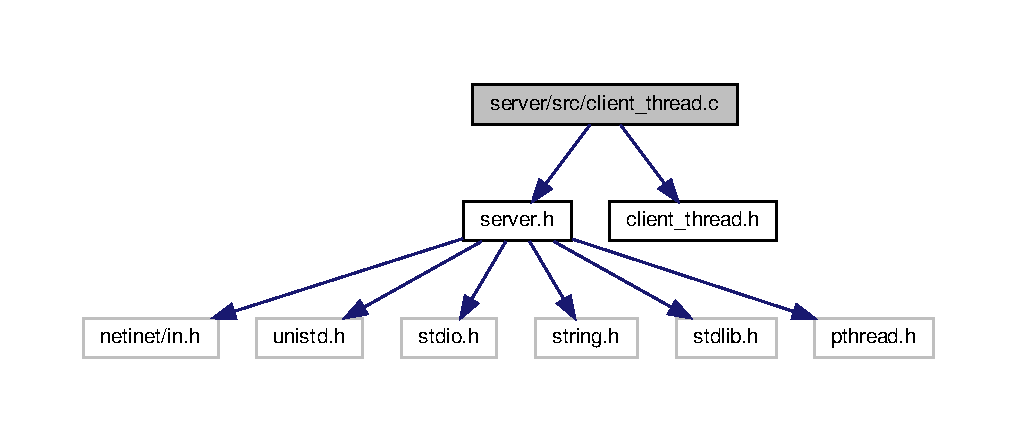
\includegraphics[width=350pt]{client__thread_8c__incl}
\end{center}
\end{figure}
\subsection*{Variáveis}
\begin{DoxyCompactItemize}
\item 
\mbox{\Hypertarget{client__thread_8c_a43fa9860b35567cb80937bd816df385f}\label{client__thread_8c_a43fa9860b35567cb80937bd816df385f}} 
\hyperlink{server_8h_a4ec25c3351f43b6c631aedeb9e14d46a}{Game} {\bfseries tictactoe} \mbox{[}N\+R\+O\+\_\+\+P\+A\+R\+T\+I\+D\+A\+S\+\_\+\+S\+I\+M\+U\+L\+T\+A\+N\+E\+AS\mbox{]}
\item 
\mbox{\Hypertarget{client__thread_8c_a0abaf4b5d42c4e5d19190035fade3599}\label{client__thread_8c_a0abaf4b5d42c4e5d19190035fade3599}} 
pthread\+\_\+mutex\+\_\+t {\bfseries lock}
\end{DoxyCompactItemize}


\subsection{Descrição Detalhada}
Implementação das funções de conexão via thread dedicada. 

\begin{DoxyAuthor}{Autor}
Vitor Correa da Silva 
\end{DoxyAuthor}
\begin{DoxyDate}{Data}
29 May 2020 
\end{DoxyDate}

\hypertarget{server_8c}{}\section{Referência do Arquivo server/src/server.c}
\label{server_8c}\index{server/src/server.\+c@{server/src/server.\+c}}


Implementação das funções do servidor.  


{\ttfamily \#include $<$server.\+h$>$}\newline
{\ttfamily \#include $<$client\+\_\+thread.\+h$>$}\newline
Gráfico de dependência de inclusões para server.\+c\+:
\nopagebreak
\begin{figure}[H]
\begin{center}
\leavevmode
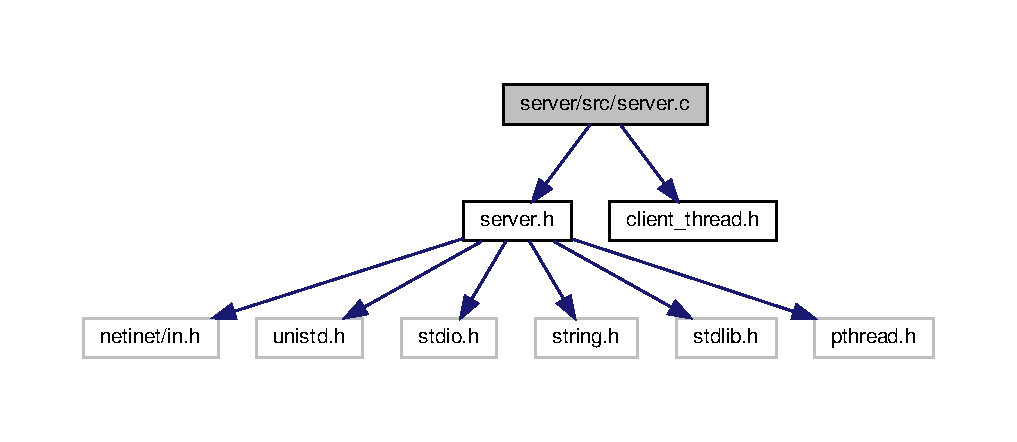
\includegraphics[width=350pt]{server_8c__incl}
\end{center}
\end{figure}
\subsection*{Funções}
\begin{DoxyCompactItemize}
\item 
void \hyperlink{server_8c_a0a489ba30d8a8b9903c80eccf0384f3b}{show\+\_\+usage} (char $\ast$bin\+\_\+name)
\begin{DoxyCompactList}\small\item\em Exibe mensagem de utilização. \end{DoxyCompactList}\item 
int \hyperlink{server_8c_a3c04138a5bfe5d72780bb7e82a18e627}{main} (int argc, char $\ast$$\ast$argv)
\begin{DoxyCompactList}\small\item\em Função main do servidor. \end{DoxyCompactList}\end{DoxyCompactItemize}


\subsection{Descrição Detalhada}
Implementação das funções do servidor. 

\begin{DoxyAuthor}{Autor}
Vitor Correa da Silva 
\end{DoxyAuthor}
\begin{DoxyDate}{Data}
29 May 2020 
\end{DoxyDate}


\subsection{Funções}
\mbox{\Hypertarget{server_8c_a3c04138a5bfe5d72780bb7e82a18e627}\label{server_8c_a3c04138a5bfe5d72780bb7e82a18e627}} 
\index{server.\+c@{server.\+c}!main@{main}}
\index{main@{main}!server.\+c@{server.\+c}}
\subsubsection{\texorpdfstring{main()}{main()}}
{\footnotesize\ttfamily int main (\begin{DoxyParamCaption}\item[{int}]{argc,  }\item[{char $\ast$$\ast$}]{argv }\end{DoxyParamCaption})}



Função main do servidor. 

Realiza a leitura dos parâmetros de linha de comando, e valida-\/os. Caso os parâmetros sejam incorretos, exibe a mensagem de utilização chamando a função {\ttfamily show\+\_\+usage} 

Após isso, a função main realiza a inicialização do servidor chamando as funções {\ttfamily init\+\_\+server} e {\ttfamily init\+\_\+shared\+\_\+variables} , cria um socket e inicia a espera por logins através da função 

Caso os parâmetros sejam válidos


\begin{DoxyParams}{Parâmetros}
{\em argc} & Número de argumentos passados por parâmetro \\
\hline
{\em argv} & Array de argumentos do tipo $\ast$char \\
\hline
\end{DoxyParams}
\begin{DoxyReturn}{Retorna}
int 
\end{DoxyReturn}
\mbox{\Hypertarget{server_8c_a0a489ba30d8a8b9903c80eccf0384f3b}\label{server_8c_a0a489ba30d8a8b9903c80eccf0384f3b}} 
\index{server.\+c@{server.\+c}!show\+\_\+usage@{show\+\_\+usage}}
\index{show\+\_\+usage@{show\+\_\+usage}!server.\+c@{server.\+c}}
\subsubsection{\texorpdfstring{show\+\_\+usage()}{show\_usage()}}
{\footnotesize\ttfamily void show\+\_\+usage (\begin{DoxyParamCaption}\item[{char $\ast$}]{bin\+\_\+name }\end{DoxyParamCaption})}



Exibe mensagem de utilização. 

Exibe a mensagem de utilização\+: \begin{DoxyVerb}usage: ./server <int: port> \end{DoxyVerb}


Se o nome do binário passado por argumento for \char`\"{}./server\char`\"{}, obviamente. 
\begin{DoxyParams}{Parâmetros}
{\em bin\+\_\+name} & Nome do binário que foi executado \\
\hline
\end{DoxyParams}

%--- End generated contents ---

% Index
\backmatter
\newpage
\phantomsection
\clearemptydoublepage
\addcontentsline{toc}{chapter}{Índice}
\printindex

\end{document}
